% \documentclass-book
\documentclass[a4paper,11pt]{book}
\usepackage[utf8]{inputenc}
\usepackage{a4wide}
\usepackage[unicode]{hyperref}
\usepackage[slovene]{babel}
\selectlanguage{slovene}
\usepackage[pdftex]{graphicx} % za slike
\usepackage{setspace}
\usepackage{textcomp}
\usepackage[version=3]{mhchem}
\usepackage{booktabs} % makes nice quality tables
\usepackage{emptypage}

% \usepackage{mathptmx}
\usepackage{palatino} 
\usepackage{pxfonts}
\usepackage{charter}
\usepackage{algorithmic} % for algorithms

\usepackage{amsopn}
\DeclareMathOperator*{\argmax}{\arg\,\max}

\renewcommand{\baselinestretch}{1.2}
\newcommand{\angl}[1]{(angl. {\em #1})}
\newcommand{\comment}[1]{#1}
\newcommand{\pd}[2]{\frac{\partial#1}{\partial#2}}
\newcommand{\plogp}[2]{{#1\over #2}\log_2{#1\over #2}}
\newcommand{\ds}{\displaystyle}
\newcommand{\mean}[1]{\overline{#1}}
\newcommand{\Var}{\mathrm{Var}}
\newcommand{\tr}{\intercal}
\newcommand{\norm}[1]{\left\lVert#1\right\rVert}

\usepackage{color}
\definecolor{light-gray}{gray}{0.95}
% \newcommand{\text}{\rm}
\usepackage{listings}
\usepackage{url}
% \usepackage{program}

\newtheorem{teorem}{Teorem}

\lstnewenvironment{python}[1][]{
\lstset{
language=python,
basicstyle=\ttfamily\footnotesize\setstretch{1},
stringstyle=\color{red},
showstringspaces=false,
alsoletter={1234567890},
otherkeywords={\ , \}, \{},
keywordstyle=\color{blue},
emph={access,and,break,class,continue,def,del,elif,else,%
except,exec,finally,for,from,global,if,import,in,is,%
lambda,not,or,pass,print,raise,return,try,while},
emphstyle=\color{black}\bfseries,
emph={[2]True, False, None, self},
emphstyle=[2]\color{green},
emph={[3]from, import, as},
emphstyle=[3]\color{blue},
upquote=true,
morecomment=[s]{"""}{"""},
commentstyle=\color{red}\slshape,
emph={[4]1, 2, 3, 4, 5, 6, 7, 8, 9, 0},
emphstyle=[4]\color{blue},
literate=*{:}{{\textcolor{blue}:}}{1}%
{=}{{\textcolor{blue}=}}{1}%
{-}{{\textcolor{blue}-}}{1}%
{+}{{\textcolor{blue}+}}{1}%
{*}{{\textcolor{blue}*}}{1}%
{!}{{\textcolor{blue}!}}{1}%
{(}{{\textcolor{blue}(}}{1}%
{)}{{\textcolor{blue})}}{1}%
{[}{{\textcolor{blue}[}}{1}%
{]}{{\textcolor{blue}]}}{1}%
{<}{{\textcolor{blue}<}}{1}%
{>}{{\textcolor{blue}>}}{1},%
% framexleftmargin=1mm, framextopmargin=1mm, frame=shadowbox, rulesepcolor=\color{blue},#1
}}{}

\lstset{ %
language=Python,
basicstyle=\ttfamily\setstretch{1},
backgroundcolor=\color{light-gray}
}

% include hyperlinks
\usepackage{hyperref}

\title{Odkrivanje znanj iz podatkov \\
\small (zapiski predavateljev, samo za interno uporabo)}
\author{Blaž Zupan}
\date{\today}


\begin{document}
\maketitle
\tableofcontents

\cleardoublepage

\chapter*{Uvod}

Predmet Odkrivanje znanj iz podatkov na magistrskem študiju je nadaljevanje predmeta Uvod iz odkrivanja znanj iz podatkov iz dodiplomskega študija. Pred 2017 se je uvodni predmet imenoval Poslovna inteligenca. Pričujoči zapiski so zato nadaljevanje zapiskov iz uvodnega predmeta in s tem predpostavijo, da se je bralec z osnovnimi koncepti in terminologijo srečal že prej. Kjer temu ni tako, priporočam pregled uvodnih zapiskov.

\cleardoublepage

\chapter{Večrazredna klasifikacija}

Eden od ključnih klasifikacijskih algoritmov, ki smo jih spoznali pri uvodnih predavanjih (Poslovna inteligenca oziroma, po novem, Uvod v odkrivanje znanj iz podatkov) je bila logistična regresija. Ta na podlagi vrednosti atributov ocenjuje verjetnost ciljnega razreda. Na primer, kateri uporabniki telefonskih storitev bodo v naslednjem mesecu dni prekinili naročniško razmerje? Ali pa, kdo od zaposlenih bo v naslednjem pol leta dal odpoved? Kateri artikli iz prodajnega kataloga bodo uporabniku, ki je opisan z vektorjem značilk, všeč? Bo popoldanski avtobus številka 10 danes prišel pravočasno do končne postaje? Ciljni razred smo tu opisali z besedami (na primer odpoved razmerja, ali pa pravočasnost avtobusa), v strojnem učenju pa zanj uvedemo razredno (odvisno) spremenljivko $y$, ki ima za $i$-ti primer lahko vrednost $y^{(i)}\in\{0,1\}$, kjer je tipično $1$ ciljna vrednost razreda (dogodek se je zgodil, na primer, zaposleni je dal odpoved) in z $0$ vrednst razreda, kjer se ciljni dogodek ni zgodil (na primer, zaposleni ni dal odpovedi). Pri logistični regresiji, tako kot pri vseh drugih klasifikacijskih algoritmih, nas seveda za dani primer zanima verjetnost ciljnega razreda, torej $p(y=1|x)$.

Zgoraj smo našteli nekaj primerov, kjer je klasifikacija binarna. Torej tam, kjer imamo slučajno spremenljivko (razred), ki lahko zavzame dve vrednosti. A je za praktične primere ta omejitev precej omejujoča. Na primer, iz končnih ocen v srednji šoli bi radi napovedali, na katero fakulteto se bo dijakinja vpisala. Iz ročno zapisane pismenke oziroma njene digitalizirane slike bi radi razbrali, za kateri znak (črko) gre. Čivku bi želeli določiti primerni emotikon. Napovedali bi radi vreme (sončno, oblačno, deževno). V vseh naštetih primerih lahko razredna spremenljivka zavzame eno od možnih vrednostih. Njena zaloga vrednosti torej ni več binarna.

Naj bo število možnih vrednosti, ki jo razredna spremenljivka zavzame, enako $K$. Vrednost ciljnega razreda bomo tu zapisali torej kar z indeksom vrednosti, torej $y\in\{0,1,\ldots,K\}$. Ta zapis uporabimo zaradi enostavnejšega enačb in formalnih modelov. Pri sporazumevanju z uporabniki oziroma pri delu z uporabniško prijaznim programom pa seveda pričakujemo, da bodo vrednosti razredne spremenljivke zavzele neko opisno vrednost, oziroma da bomo lahko poročali o modelih in njihovih napovedih v obliki, ki je blizu uporabniku\footnote{Ta želja je sicer trivialna, a je mnoga, tudi popularna okolja za strojno učenje, zaobidejo. Okolje scikit-learn, na primer, zna delati samo s številskimi vrednostmi in je implementacija poročanja s simbolnimi vrednostmi prepuščena uporabniku te knjižnice oziroma razvijalcu.}.

Tu se pojavi problem. Logistična regresija je tehnika, ki lahko obravnava samo binarne probleme, torej samo probleme, kjer je razred dvovrednosten. Večvrednostnih problemov, torej problemov, kjer število vrednosti razredov presega dva, logistična regresija sama po sebi ne zna obravnavati. Omejitev na binarno klasifikacijo ni lastna samo logistični regresiji: podobno je tudi z drugimi popularnimi tehnikami, kot sta na primer metodi podpornih vektorjev in diskriminantna analiza. Po drugi strani pa smo že spoznali metode, ki so že v osnovi primerne za večvrednostno klasifikacijo. Med temi so metoda klasifikacijskih dreves, $k$-najbližjih sosedov, in klasifikacijski gozdovi.

V tem poglavju se bomo pravzaprav osredotočili na logistično regresijo in razmišljali o tem, kako to metodo prilagoditi v namene večvrednostne klasifikacije. In sicer na dva načina. Pri prvem bomo metodo samo pustili pri miru in poskušali večvrednostno klasifikacijo prevesti v binarni problem. Tehnike, ki jih bomo uporabili, bodo primerne za uporabo tudi za ostale binarne klasifikatorje. Pri drugem načinu pa bomo dejansko posegli v ogrodje logistične regresije in spremenili model tako, da bo primeren za ocenjevanje verjetnosti vrednosti večvrednostnega razreda.

\section{Ovojnica za binarne klasifikatorje}

Pri tem pristopu vzamemo binarni klasifikator, torej, metodo, ki se zna naučiti na primerih, ki pripadajo enemu od dveh razredov. Problem prilagodimo tako, da pripravimo podatke za binarno učenje, se naučimo niza binarnih klasifikatorjev in potem te združeno uporabimo za večvrednostno klasifikacijo. Dva najbolj znana, pa tudi morda najbolj enostavna pristopa sta:

\begin{description}
\item[Eden-proti-vsem.] Za vsak razred $k\in\{1,2,\ldots,$K$\}$ konstruiraj klasifikator $h_k$, tako da je $y_k=h_k({\bf X},{\bf y}_k)$, kjer je vrednost vektorja razrednih vrednosti $y_k$ za $i$-ti primer enaka:
  $$
  {y_k^{(i)}}=
  \begin{cases}
    1, & \text{if } y^{(i)}\equiv k \\
    0, & \text{otherwise}
  \end{cases}
  $$
  Ko dobimo primer, za katerega moramo napovedati vrednost razreda in ki ga opišemo z vektorjem atributov $x$, uporabimo vse razvite modele $h_k$ in napovemo vrednost razreda $k$ za model, ki napove največjo verjetnost razreda 1. Torej:
  $$\hat{y}=\argmax_{k=1\ldots K} h_k(x)$$
\item[Eden proti drugemu.] Naučimo se $k(k-1)/2$ klasifikatorjev $h_{a,b}$ za vsak par $(a,b)$ razredov. Pri napovedi uporabimo vse klasifikatorje in izberemo razred, ki je bil največkrat napovedan oziroma je največkrat zmagal.
\end{description}

Zgoraj smo opisali napovedovanja razredne vrednost, ne pa tudi postopke ocenjevanja njihovih verjetnosti. Bolj za silo in ne preveč formalno poglobljeno se da zgornja postopka prirediti tudi tako, da napovedujeta verjetnosti. In sicer, za postopek eden-proti-vsem tako, da za razredne verjetnosti vzamemo napovedane verjetnosti $h_k(x)$ ter jih normaliziramo, pri postopku eden-proti-drugemu pa ocenimo verjetnosti tako, da so te proporcionalne številu napovedi, kjer je določen razred zmagal. Ali pa so morda proporcionalne povprečni verjetnosti, s katero je bil ocenjen razred pri klasifikatorju, ki je ta razred vseboval. Kot rečeno, so vsi ti prijemi sicer inženirski in precej {\em ad hoc} in bi nam koristilo kaj boljšega, z nekaj več formalne podlage. O tem v nadaljevanju.

\section{Nekaj razmišljanj o logistični regresiji}

Še enkrat si poglejmo si logistično regresijo (za njeno izpeljavo glej zapiske pri predmetu Uvod v odkrivanje znanj iz podatkov), tokrat iz malce bolj inženirskega vidika. Logistična regresija v osnovi predpiše vsakemu primeru neko število iz intervala $(-\infty,+\infty)$. Vrednost atributov primera hranimo v vektorju $x$, za preslikavo iz atributnega prostora v prostor realnih števil pa bomo uporabili neko funkcijo, recimo $f(x)$. Število, ki nam ga vrne funkcija $f(x)$ logistična regresija potem pretvori v verjetnost ciljnega razreda, to je verjetno $p(y=1|x)$. Verjetnosti so omejene na vrednosti med $0$ in $1$. Funkcija, ki je primerna za tako pretvorbo, je logistična:
%
$$ g(z)=\frac{1}{1+e^{-z}} $$

Logistični model oziroma verjetnost ciljnega razreda je torej $\hat{y}=g(f(x))$. Opazimo lahko, da je $g(-\infty)=0$ in da je $g(+\infty)=1$, ter da je $g(0)=0.5$. Za primere v ciljnem razredu bi bilo torej dobro, da nam $f(x)$ vrača pozitivne, čim večje vrednosti, za primere v neciljnem razredu pa negativne, torej čim manjše vrednosti. Najbrž najbolj enostavna funkcija, ki izračuna $f(x)$ (spomnimo: x je vektor atributnih vrednosti) je linearna: $f(x)=\sum \theta_i x_i$. In prav to, linearno funkcijo, uporablja logistična regresija. Če bi bil vektor parametrov modela $\Theta$ enotski vektor, bi $f(x)$ vračala razdaljo primera do premice, ki jo določajo parametri $\Theta$. Ker pa ne zahtevamo enotske dolžine tega vektorja na zahtevamo, lahko rečemo le, da je $f(x)$ premosorazmerna razdalji do premice. Kar je popolnoma v redu, saj enot, v katerih so zapisani atributi ne poznamo, in nam dejanska razdalja v izbranih enotah ne pove ničesar.

Oglejmo si to na primeru. Slika~\ref{f:lr-margin} prikazuje primere v dvo-atributnem prostoru in ločnico ($f(x)$) med njimi, ki smo jo dobili z logistično regresijo. Bolj, kot so točke oddaljene od ločnice, večja je verjetnost, da pripadajo enemu ali drugemu razredu. Idealno bi bilo, da je linearna ločnica taka, da loči vse točke enega razreda od točk drugega razreda. V našem primeru taka ločnica ne obstaja, zato logistična regresija nekatere primere iz učne množice razvrsti napačno.

\begin{figure}[htbp]
\centering{
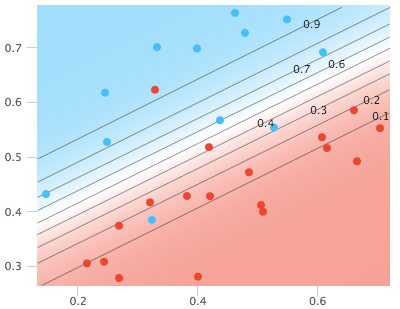
\includegraphics[width=10cm]{slike/logisticna-regresija-konture.png}
\caption{Podatki v prostoru dveh atributov in ločitvena meja med razredi, ki jo uporablja model logistične regresije.}
\label{f:lr-margin}}
\end{figure}

\section{Večrazredna logistična regresija}

Postopek, ki ga bomo tu opisali, se imenuje tudi regresija softmax \angl{softmax regression}\footnote{Pri izpeljavi regresije softmax smo se zgledovali po spletni strani \url{http://ufldl.stanford.edu/tutorial/supervised/SoftmaxRegression/}.}. Nazivi so sicer rahlo zavajajoči, saj gre za klasifikacijsko in ne regresijsko metodo, a po drugi strani čisto informativni, saj v jedru uporabljajo linearno kombinacijo atributov. Za logistično regresijo smo zgoraj omenili, da pretvori atributni vektor $x$ v neko število $f(x)$, tega pa potem v verjetnost ciljnega razreda. Pri večrazredni, tudi imenovani multinomski klasifikaciji, bi lahko izhajali iz predpostavke, da smo za nek atributni vektor za vsakega od razredov izračunali neko število. Recimo, napovedujemo vreme: jasno, oblačno ali deževno. Predstavljajmo si, da imamo nek predpis, ki nam iz dnevne karte Slovenije (vektor atributov) izračuna vektor števil za naš tri razrede. Naj bo ta vektor $z=[2.5, 3.7, 1.9]^T$. Naj nas tu zaenkrat ne bega, kako smo do tega vektorja prišli, a vsekakor opazimo, da to niso verjetnosti. Verjetnosti pa so ravno tiste, ki bi jih od našega napovednega modela želeli. Potrebujemo predpis, funkcijo, ki naš vektor pretvori v verjetnosti, torej predpis, ki stori nekaj z vektorjem $z$ tako, da iz njena izračuna vektor istih dimenzij, kjer so vrednosti verjetnosti razredov, ki se seveda seštejejo v 1. Tak predpis je funkcija softmax:

$$\sigma(z_j) = \frac{e^{z_j}}{\sum_{k=1}^K e^{z_k}}$$

Softmax nam torej naš vektor $z=[2.5, 3.7, 1.9]^T$ pretvori v vektor
$\sigma(z)=[0.21, 0.68, 0.11]$. Funkcija sama poskrbi, da je vektor enotni, saj elemente vektorja ($e^{z_j}$) v funkcijskem predpisu deli z njihovo vsoto, torej jih normira.

V redu. A kako dobimo elemente vektorja $z$? Tako kot pri logistični regresiji, naj bo tudi ta izračunan z linearno kombinacijo atributnih vrednosti. Za $j$-ti razred in vektor atributnih vrednosti $x$ zapišemo torej:

$$ z_j(x)=\theta_{j,0}+\theta_{j,1} x_1 + \ldots + +\theta_{j,n} x_n $$

Z $n$ smo tu označili število atributov. Za bolj kompakten zapis se dogovorimo, kot smo to storili pri logistični regresiji, da uvedemo še $x_0=1$. Vektorski zapis zgornje linearne kombinacije je:

$$ z_j(x) = \Theta_j^T x $$

Naš mutlinomiski logistični model bo torej za primer opisan z vektorjem atributnih vrednosti $x$ vračal vektor verjetnosti, kjer bo posamezen element ustrezal verjetnosti posameznemu razredu:

\begin{equation}
  \nonumber
  h_\Theta(x) =
  \begin{bmatrix}
    p(y=1|x;\Theta_1) \\ p(y=2|x;\Theta_1) \\ \vdots \\ p(y=k|x;\Theta_k)
  \end{bmatrix}
  = \frac{1}{\sum_{j=1}^{k}e^{\Theta_j^T x}}
  \begin{bmatrix}
    e^{\Theta_1^T x} \\ e^{\Theta_2^T x} \\ \vdots \\ e^{\Theta_k^T x}
  \end{bmatrix}
\end{equation}

Za razred $j$ in primer $x$ je torej verjetnost razreda:

$$ p(y=j|x;\Theta_j)=\frac{e^{\Theta_j^T x}}{\sum_{k=1}^K e^{\Theta_k^T x}} $$

Pozor: $\Theta_1$, $\Theta_2$ do $\Theta_k$ so vektorji in parametri modela, posamezen vektor parametrov za posamezen razred. Da bo vse skupaj bolj kompaktno, te parametre lahko združimo v matriko $\Theta$:

\newcommand{\myrule}{\rule[.5ex]{2em}{0.4pt}}

$$
\Theta =
\begin{bmatrix}
  \myrule~\Theta_1^T~\myrule \\ 
  \myrule~\Theta_2^T~\myrule \\
  \vdots \\
  \myrule~\Theta_k^T~\myrule
\end{bmatrix}
$$

Zgoraj smo določili strukturo modela. Model sam pa bo odvisen od vrednosti parametrov modela, torej vrednosti elementov matrike $\Theta$. Te vrednosti moramo določiti tako, da se bo model čim bolje prilegal učnim podatkom, torej podatkom zbranih v matriki atributov $X$ in vektorju razredov $y$. Prileganje moramo opisati kvantitativno, torej določiti cenovno funkcijo $J(\Theta)$. Do te pridemo preko verjetja. Torej, kakšna je verjetnost, da bomo z našim modelom, ki ga določajo parametri $\Theta$, napovedali pravo vrednost razredov:

\begin{equation}
  \begin{split}
    L(\Theta) & = p(y|X;\Theta) \\
    & = \prod_i^m p(y^{(i)}|x^{(i)};\Theta)
  \end{split}
\end{equation}

Verjetje želimo maksimizirati, torej izbrati take parametre $\Theta$, kjer je verjetje največje. Isto enačbo za verjetje smo že videli (poglej poglavje o logistični regresiji). Tudi takrat smo potožili, da je s produkti delati težko in da so vsote bolje. Nič se ne bo spremenilo, če namesto verjetja uporabimo logaritem verjetja:

\begin{equation}
  \begin{split}
    l(\Theta) & = \log L(\Theta) \\
    & = \sum_i^m p(y^{(i)}|x^{(i)};\Theta)
  \end{split}
\end{equation}

Knjižnice z optimizacijskimi funkcijami tipično iščejo minimume. Naša cenovna funkcija bo zato:

\begin{equation}
  \begin{split}
    J(\Theta) & = -l(\Theta) \\
    & = - \log \sum_i^m p(y^{(i)}|x^{(i)};\Theta) \\
    & = \sum_{i=1}^{m} \log\frac{\exp(\theta_{y^{i}}^T x^{(i)})}{\sum_{j=1}^K \exp(\theta^{(j)\top} x^{(i)})} \\
    & = \sum_{i=1}^{m} \sum_{k=1}^{K}  1\left\{y^{(i)} = k\right\} \log \frac{\exp(\theta^{(k)\top} x^{(i)})}{\sum_{j=1}^K \exp(\theta^{(j)\top} x^{(i)})}
  \end{split}
\end{equation}

Zgornja notacija z $\theta_{y^{i}}^T$ je malce čudna, a pomeni, da izberemo tisti $\theta$ vektor, ki ustreza razredu $y^{i}$. To je z vsoto in indikatorsko funkcijo morda še bolj čudno zapisano v naslednji vrstici. Indikatorska funkcija $1\left\{y^{(i)} = k\right\}$ vrne vrednost 1, če je izraz v oklepajo resničen, sicer pa vrednost 0. A je od vseh zapisov prav ta v zadnji vrstici najbolj uporaben. Verjetnosti v imenovalcu moramo tako ali tako izračunati. Shranimo jih v matriki. Potem iz matrike za števec izberemo samo tiste vrednosti, ki dejansko ustrezajo razredu $i$-tega primera.

Kriterijsko funkcijo imamo. Za izračun parametrov modela bomo uporabili gradientni sestop, oziroma katerokoli (boljšo) optimizacijsko metodo, ki pa potrebuje izračun gradienta. Ta je za $k$-ti vektor parametrov, torej za parametre, ki ustrezajo $k$-temu razredu, enak:

\begin{equation}
\nabla_{\Theta_k} J(\Theta) = - \sum_{i=1}^{m}{ \left[ x^{(i)} \left( 1\{ y^{(i)} = k\}  - p(y^{(i)} = k | x^{(i)}; \Theta) \right) \right] }
\end{equation}
%
Poiskati moramo vrednosti parametrov, ki zgornji izraz minimizirajo. Izraz v notranjem oklepaju gre za primere razreda $k$ proti vrednosti 0, če je le ocenjena verjetnost za ta razred visoka (1 minus nekaj, kar gre proti 1, gre skupaj proti 0). Za primere, ki niso v razredu $k$, pa pričakujemo, da je verjetnost tega razreda čim manjša.

Od tu dalje je enostavno. Lahko uberemo metodo gradientnega sestopa in neko začetno matriko $\Theta$ (morda tako, kjer so vse vrednosti enake 0) osvežujemo:

$$ \Theta_k\leftarrow\Theta_k-\alpha\nabla_{\Theta_k} J(\Theta) $$
%
ali pa (bolje) uporabilo postopek kot je L-BFGS iz za to dostopne knjižnice.

\section{Predoločenost}

Model, ki smo ga uvedli zgoraj, je predoločen. Ima preveč parametrov. Rešitev za $\Theta$ je poljubno mnogo. Zakaj? Vzemimo, da vse vektorjem $\Theta_k$ odštejemo nek poljuben vektor $\Psi$:

\begin{equation}
\begin{split}
p(y = k | x ; \theta)
&= \frac{\exp((\theta_k-\psi)^T x)}{\sum_{j=1}^K \exp( (\theta_j-\psi)^T x)}  \\
&= \frac{\exp(\theta_k^T x) \exp(-\psi^T x)}{\sum_{j=1}^K \exp(\theta_j^T x) \exp(-\psi^T x)} \\
&= \frac{\exp(\theta_k^T x)}{\sum_{j=1}^K \exp(\theta_j^T x)}.
\end{split}
\end{equation}

Hm. Torej odštevanje vektorja $\Psi$ ne vpliva prav nič in se iz vseh enačb pokrajša. Torej, lahko vstavimo, da je $\Psi=\Theta_1$ in je potem $\Theta_1-\Psi=0$. Torej, prva vrstica v matriki $\Theta$ ima vse vrednosti nastavljene na nič. In je pri optimizaciji sploh ne rabimo računati. Računamo potem vse ostale vrednosti. Namesto začetnih $k\times(n+1)$ parametrov imamo tako sistem z $(k-1)\times(n+1)$ parametrov. In eno samo rešitev.

\section{Večrazredna in dvorazredna logistična regresija}

Premislimo, kaj je z večrazredno logistično regresijo v posebnem primeru, ko je $K=2$. Naš vektor verjetnosti razredov bo:

\begin{equation}
\begin{split}
h_\Theta(x) & =
\frac{1}{\exp(\Theta_1^T x)  + \exp(\Theta_2^T x ) }
\begin{bmatrix}
\exp( \Theta_1^T x ) \\
\exp( \Theta_2^T x )
\end{bmatrix}
\end{split}
\end{equation}

Ta sistem, kot vemo iz prejšnjega razdelka, je predoločen. Izberemo vektor $\Psi=\Theta_1$ in ga odštejemo od $\Theta_1$ in $\Theta_2$:

\begin{equation}
\begin{split}
h(x) & =
\frac{1}{ \exp( (\theta_1-\theta_2)^T x^{(i)} ) + \exp(\vec{0}^T x) }
\begin{bmatrix}
\exp( (\theta_1-\theta_2)^T x )
\exp( \vec{0}^T x ) \\
\end{bmatrix} \\
& =
\begin{bmatrix}
\frac{1}{ 1 + \exp( (\theta_1-\theta_2)^T x ) } \\
\frac{\exp( (\theta_1-\theta_2)^T x )}{ 1 + \exp( (\theta_1-\theta_2)^T x ) }
\end{bmatrix} \\
& =
\begin{bmatrix}
\frac{1}{ 1  + \exp( (\theta_1-\theta_2)^T x ) } \\
1 - \frac{1}{ 1  + \exp( (\theta_1-\theta_2)^T x ) } \\
\end{bmatrix}
\end{split}
\end{equation}

V zgornji enačbi nadomestimo $\theta_1-\theta_2$ z $\theta$ in dobimo identični model kot pri logistični regresiji. Regresija softmax pri $K=2$ je identična logistični regresiji.

\section{Regularizacija}

Tako, kot se logistična regresija lahko preveč prilagodi učnim podatkom, to velja tudi za mutlinomsko regresijo. Preveliko prilaganje pomeni visoke vrednosti v matriki $\Theta$ (to vemo že iz linearne regresije, pa tudi iz logistične; oboje iz lekcije o polinomski razširitvi učnih primerov). Zdravilo te anomalije je regularizacija. Cenovna funkcija z regularizacijo je:

\begin{equation}
\nabla_{\Theta_k} J(\Theta) = - \sum_{i=1}^{m}{ \left[ x^{(i)} \left( 1\{ y^{(i)} = k\}  - p(y^{(i)} = k | x^{(i)}; \theta) \right) \right] } + \frac{\lambda}{2}\sum_{k=1}^K\sum_{j=1}^n\Theta_{kj}^2
\end{equation}

Gradient se nam skladno z zgornjo spremembo poveča za $\lambda\Theta_k$.

\cleardoublepage

\chapter{Ocenjevanje in izbor atributov}

Ocenjevanje in izbor atributov sta osnovni opravili vsakega podatkovnega rudarja. Namreč, odkrivanje znanj iz podatkov temelji na tem, da ugotovimo, kateri atributi pomembni in prevladujoče vplivajo na obnašanje modela, kakršenkoli naj slednji bo. V tem poglavju se bomo sicer s primerom omejili na klasifikacijske probleme, a je koncepte, ki jih bomo spoznali, prav enostavno razširiti na kakršenkoli drugo nalogo.

Ocenjevanje informativnosti atributov je predvsem pomembno takrat, ko želimo podatke in iz teh porajajoče se modele razumeti. Na primer, želimo vedeti, kateri od atributov, s katerim opišemo naročnika mobilnih storitev, je tisti, ki je najbolj povezan z prekinitvijo naročniškega razmerja. Ali pa, v medicini, kateri od simptomov je najbolj povezan z diagnozo, ali pa prognozo. Morda celo, katere so tiste ključne besede v čivkih, ki so povezane s tečajem določene valute.

Z ocenjevanjem informativnosti atributov je povezan tudi njihov izbor. V splošnem bi iz začetne množice atributov, s katerimi smo popisali primere, radi izbrali množico atributov, ki je po nekem kriteriju najboljša. Recimo tako, na podlage katere nam izbrana metoda strojnega učenja zgradi model z visoko napovedno točnostjo. Na podlagi stopnje povezanosti oziroma vključenosti ocenjevanja v izgradnjo modelov tudi ločimo tri različne načine izbora atributov:
%
\begin{enumerate}
\item {\bf Filter}. Atributom pripišemo stopnjo informativnosti, ki jo izračunamo neposredno iz podatkov. Pri tem lahko upoštevamo samo vrednosti atributa in razreda (univariatni pristop) ali pa kontekst, torej tudi vrednosti ostalih atributov (multivariatni pristop). Predvsem univariatne metode so lahko izjemno časovno učinkovite, a je tu težava pri določanju praga, koliko atributov izbrati. Kratkovidnost univariatnih metod rešujemo z multivariatnimi pristopi (npr. metoda Relief), ki pa so časovno potratnejše. Tudi pri njih ostaja problem, koliko atributov izbrati.
\item {\bf Ovojnica}. Atribute izberemo tako, da optimiziramo napovedno točnost modelov. Tipično zberemo neko začetno množico atributov, preverimo napovedno točnost modela, ki ga zgradimo na tej množici, in tej množici dodajamo ali odvzemamo atribute s ciljem izboljšanja točnosti. Metode te vrste so tipično časovno potratne.
\item {\bf Metoda učenja.} Veliko metod strojnega učenja z uteževanjem ali kar neposredno z uporabo samo nekaterih atributov na ta način, torej znotraj metode, vrši izbor značilk. Primer takih tehnik so regresijska in klasifikacijsko drevesa, naključni gozdovi ter linearna in logistična regresija. Pri slednjih je še posebej zanimiva kombinacija z regularizacijo L1.
\end{enumerate}

Obstaja vrsta odličnih pregledov različnih vrst in tipov zgoraj omenjenih metod. Cilj tega poglavja je samo osnovni pregled, morda še ožje, relacija med izborom značilk in nevarnostjo, da se z njo preveč prilagodimo podatkom. A pojdimo po vrsti in pričnimo s primerom.

\section{Primer podatkov}

Za primer si poglejmo podatke, iz katerih lahko morda ugotovimo, ali ima kajenje sploh kakšne posledice. Recimo, na [limfocite](https://sl.wikipedia.org/wiki/Limfocit), to je na vrsto belih krvnih telesc. Še najbolj sistematično lahko posledice kajenja opazujemo tako, da pogledamo, kaj se dogaja v celicah limfocitov. Biologi danes dogajanja v celicah opazujejo tudi preko izražanja vseh genov v celici (človekov genom jih ima okoli $20.000$). To je, z meritvami, koliko so geni aktivni pri proizvajanju proteinov. Še bolj direktno bi stanje v celici lahko ocenili s koncentracijo vseh proteinov, a je ta tehnologija dražja in manj dostopna. Tu nas je morda malce zaneslo pri domeni vsled piščeve navdušenosti nad biotehnolgoijo, ampak na koncu je enostavno: imamo primere (79 žensk, med njimi 40 kadilk in 39 nekadilk) in meritve izražanj $14.093$ genov v njihovih limfocitih (atributi). Podatki so prosto dostopni v zbirki GEO Data Sets~\footnote{\url{https://www.ncbi.nlm.nih.gov/sites/GDSbrowser?acc=GDS3713}}. Naš cilj je ugotoviti, koliko atributov nam pove kaj o razredu. Oziroma, po biološko, koliko je takih genov, katerih izražanje se spremeni pri kadilkah.

\section{Ocenjevanje informativnosti}

Pod informativnost tu razumemo povezanost med vrednostjo atributa in razredom. Z drugimi besedami, v kakšni meri lahko iz vrednosti atributa napovemo razred. Kot kaže slika~\ref{f:fss-instance-dist}, so lahko atributi bolj ali manj povezani z razredom.

\begin{figure}[htbp]
\centering{
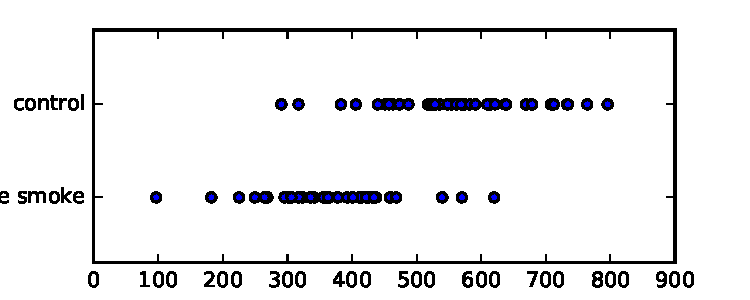
\includegraphics[width=10cm]{slike/fss-informative.pdf}
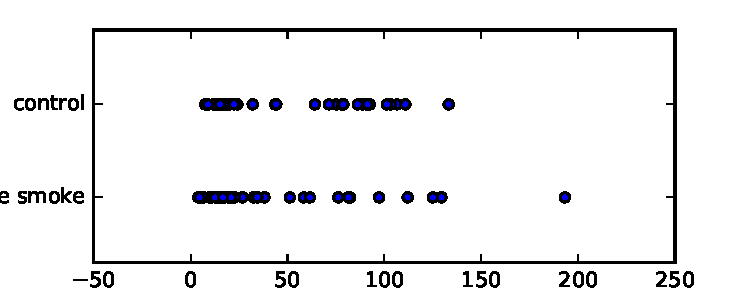
\includegraphics[width=10cm]{slike/fss-noninformative.pdf}
\caption{Porazdelitev vrednosti informativnega (zgoraj) in neinformativnega (spodaj) atributa pri primerih v prvem (``control'') in drugem razredu (``cigarette smoke'').}
\label{f:fss-instance-dist}}
\end{figure}

Pri zveznih atributih in diskretnem razredu za informativen atribut pričakujemo, da bo ta zavzel podobne vrednosti pri primerih istega razreda, ki bodo drugačne od vrednosti atributov za primere ostalih razredov. Za binarno klasifikacijo nam to razliko dobro kvantificira Studentovo t-statistika za ocenjevanje razlik med dvema skupinama meritev $X_0$ in $X_1$, kjer so v matriki $X_0$ zapisane atributne vrednosti primerov enega razreda ($y=0$) in v matriki $X_1$ atributne vrednosti primerov drugega razreda ($y=1$). Želimo torej, da bi bila povprečna vrednost med tema skupinama čim bolj drugačna, torej absolutna razlika med njima čim večja, ter da bi razsipanje vrednosti znotraj skupin bilo čim manjše. Pri slednjem bi bilo dobro upoštevati tudi število primerov v posamezni skupine. Vse skupaj strnemo v enačbo za že omenjeno t-statistiko:

$$t=\frac{\mean{X_0}-\mean{X_1}}{\sqrt{\ds\frac{s_0^2}{n_0}+\frac{s_1^2}{n_1}}}$$

kjer sta $s_0$ in $s_1$ standardna odklona vzorcev $X_0$ in $X_1$. Zanima nas povprečna vrednost t-statistike, torej $|t|$. Za naš primer kadilk in nekadilk je porazdelitev vrednosti te statistke, torej vrednosti ocen informativnosti atributov takšna, kot jo prikazuje slika~\ref{f:fss-score-dist-true}.

\begin{figure}[htbp]
\centering{
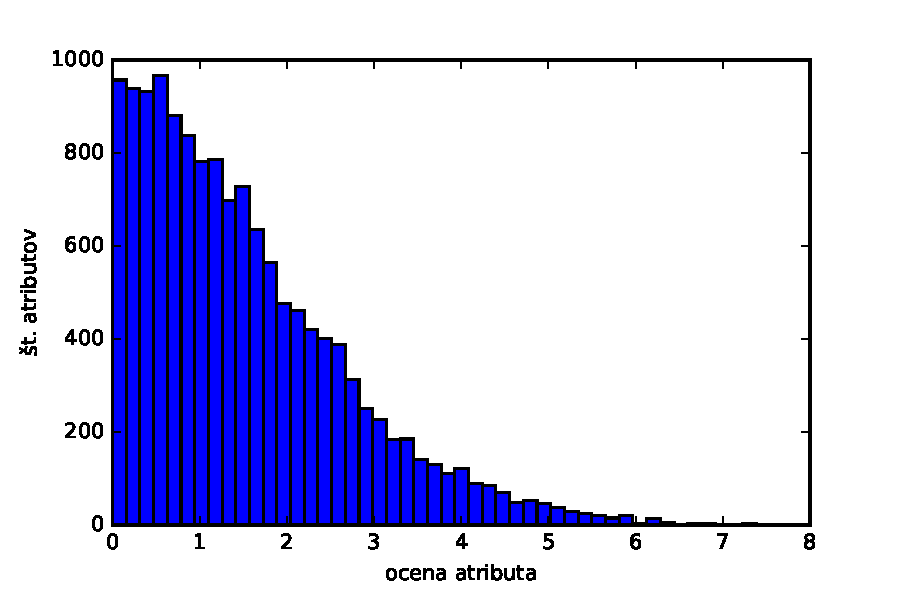
\includegraphics[width=10cm]{slike/fss-score-dist-true.pdf}
\caption{Porazdelitev ocen informativnosti atributov.}
\label{f:fss-score-dist-true}}
\end{figure}

Tu je na mestu opozorilo. Zgoraj smo uvedli eno od metod za univariatno ocenjevanje informativnosti atributov. Ta je priročna samo v primeru, ko je atribut zvezen, razred pa binaren. V primeru večvrednostnega razreda bi bilo potrebno uporabiti statistiko ANOVA. Če bi bili atributi diskretni, bi lahko uporabili informacijski prispevek, ali pa $\chi^2$. Univariantnih za različne kombinacije tipov atributov in razredov je veliko in bi bilo naštevanje na tem mestu neprimerno enciklopedično. Raje nadaljujmo z vprašanjem, kaj nam sploh ocene atributov povedo oziroma kateri atributi so potem sploh povezani z razredom. Ali bolje, kje, na sliki~\ref{f:fss-score-dist-true} je meja, od katere naprej bi lahko trdili, da je atribut informativen.

\section{Permutacijski test}

Naši podatki vsebujejo veliko število atributov in relativno majhno število primerov. Prav lahko bi se zgodilo, da je kakšen od teh atributov informativen popolnoma naključno, torej, da so meritve bile slučajno take, da so ravno dovolj ločile izbrani dve skupini oziroma razreda. Kakšna bi bila potem porazdelitev atributnih ocen, torej porazdelitev, če bi bile meritve naključne meritvah? Ali pa, če bi laborant pomešal oznake vzorcev in bi bili razredi primerov napačni. Do naključnih meritev lahko pridemo tako, da vrednosti za dani atribut premešamo, še lažje pa to storimo za vse atribute naenkrat tako, da premešamo vrednosti razredne spremenljivke. Po tej permutaciji ocenimo informativnost atributov. Da vse skupaj ne bo odvisno od ene same permutacije razredov, lahko postopek nekajkrat ponovimo. Za naše podatke in oceno s t-statistiko dobimo porazdelitev ocen, kot nam jo prikazuje graf na sliki~\ref{f:fss-score-dist-null}.

\begin{figure}[htbp]
\centering{
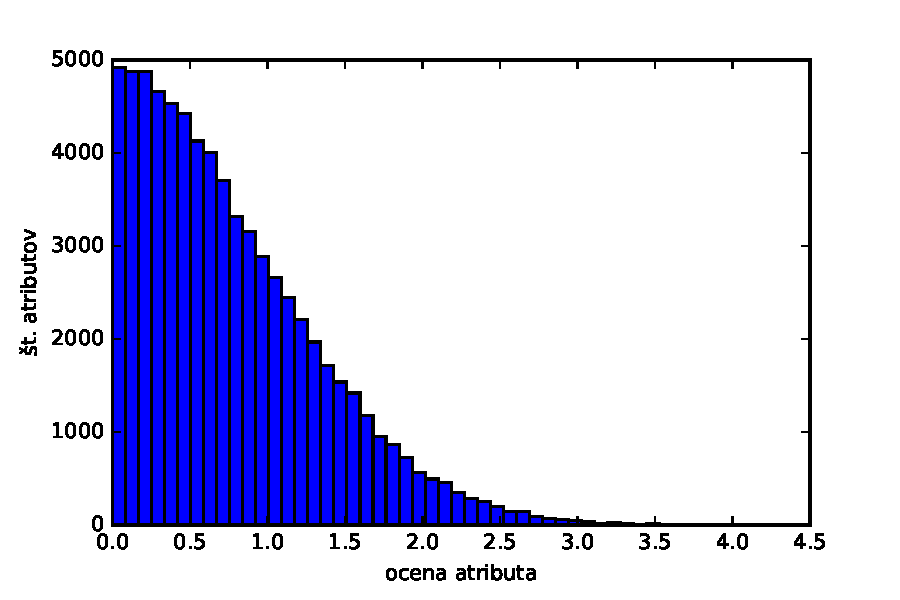
\includegraphics[width=10cm]{slike/fss-score-dist-null.pdf}
\caption{Porazdelitev ocen informativnosti atributov, ki smo jih dobili na ``pokvarjenih'' podatkih, kjer smo premešali vrednosti razredne spremenljivke oziroma premetali kolono z razredom.}
\label{f:fss-score-dist-null}}
\end{figure}

Porazdelitev ocen informativnosti atributov, ki jih izračunamo nad ponaključenimi podatki, je dosti ožja od te pridobljene iz originalnih, ``nepokvarjenih'' podatkov. Slika~\ref{f:fss-score-dist-both} nam prikazuje obe distribuciji hkrati. Na njej smo z navpično nakazali na mejo, od katere dalje je na permutiranih podatkih zelo majhno število ocen oziroma je delež takih meritev samo $p=0.001$. Za vse atribute, ki so bili ocenjeni desno od te meje, lahko trdimo, da je vrednost njihove ocene taka, da bi jo težko dobili na naključnih podatkih. Verjetnost, da bi se to lahko zgodilo, je enaka vrednosti $p$, na podlagi katere smo mejo določili. Če bi radi to verjetnost še zmanjšali, ustrezno zmanjšamo vrednost $p$. Koliko je sploh takih atributov? Za našo izbrano vrednost meje oziroma napake $p$ je takih 1327 atributov, se pravi, nekako desetina vseh genov, ki so bili vključeni v meritve. Pri veliko strožji meji, na primer $p=0.0001$, se število takih atributov zmanjša na 734.

\begin{figure}[htbp]
\centering{
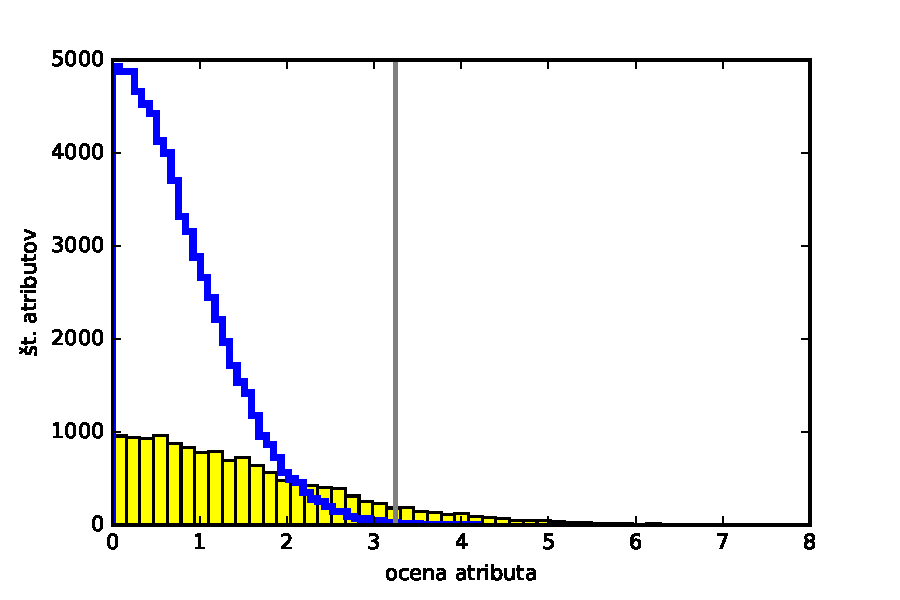
\includegraphics[width=10cm]{slike/fss-score-dist-both.pdf}
\caption{Primerjave porazdelitve ocen informativnosti atributov na ponaključenih podatkih (rumena črta) in pravih podatkih (histogram v modrem).
Siva navpičnica nakazuje mejo, od katere desno je samo zelo majhen delež ocen ($p=0.001$), ki so bile pridobljene na naključnih podatkih. 
}
\label{f:fss-score-dist-both}}
\end{figure}

V podatkih je torej samo približno desetina atributov, za katere kaže, da so povezani z razredom. To je pravzaprav za naš problem zelo veliko. Spomnimo se, preučujemo učinke kajenja in kot vse kaže obstaja kar ena desetina vseh opazovanih genov, katerih izražanje v limfocitih se zaradi kajenja spremeni.

Seveda se tu lahko vprašamo, kakšna meja je smiselna, oziroma kakšna je smiselna verjetnost napake, s katero trdimo, da je atribut informativen, čeprav bi lahko njegovo kvantitativno vrednost informativnost dobili tudi na naključnih podatkih. Odgovora za to ni. Vrednost $p$ je pač nek parameter, katerega intuitivno interpretacijo smo podali zgoraj, nekega pravila zanj pa ni. Meja, ki smo jo postavili zgoraj, torej $p=0.001$, je tipično dovolj ostra, da na realnih primerih z uporabo nje dobimo z razredom dobro povezane atribute.

\section{Izbor atributov}

Zgoraj smo ravno pridelali metodo za ocenjevanje in izbor značilk po principu filtriranja. Ocenjevanje nam pomaga pri razpoznavi tistih značilk, ki so za naš problem pomembne. Če bi bili biologi, bi nas seznam genov, ki so najbolj različno izraženi pri dveh skupinah (kadilke, nekadilke) močno zanimali. A nismo, tako da bomo tu razlago izbranih atributov zaenkrat preskočili (se boste pa s tem pozabavili pri domači nalogi na problemu, kjer bo informativnost značilk moč enostavno interpretirati). Tu razmislimo o drugačni uporabi filtriranja značilk. In sicer, v povezavi z napovednimi modeli. Ideja je, da lahko dober izbor značilk pomaga h gradnji bolj točnih modelov, ali pa vsaj pomaga k poenostavitvi problema tako, da so lahko ti odvisni od manj parametrov in jih je zato hitreje naučiti in se morda lahko manj prilegajo k učnim podatkom.

Za poskus, ali zgornje drži, naredimo nekaj poskusov. Pri prvem izberimo manjši nabor najbolj informativnih značilk in z prečnim preverjanjem ocenimo kvaliteto napovednih modelov na tako pridobljenih podatkih. Rezultate kaže tabela~\ref{t:fss-cv-false}.

\begin{table}[htbp]
  \begin{center}
    \begin{tabular}{rrr}
      \toprule
      atributov & log. reg. & k-NN \\
      \midrule
      14093 & 0.924 & 0.721 \\
      1000 & 0.936 & 0.886 \\
      100 & 0.924 & 0.873 \\
      10 & 0.784 & 0.886 \\
      \bottomrule
    \end{tabular}
  \end{center}
  \caption{Klasifikacijska točnost logistične regresije in metode najbližjih sosedov ocenjena s prečnim preverjanjem pri podatkih, kjer smo pred prečnim preverjanjem izbrali najbolj informativne atribute.}
  \label{t:fss-cv-false}
\end{table}

Zanimivo. Dobre točnosti lahko dosežemo že na podatkih, ki vsebujejo veliko (veliko!) manjše število atributov. Točnost metode najboljših sosedov se z izborom celo poveča.

Pa je naš pristop res pravi? Naredimo (en malce odštekan) eksperiment. Uničimo podatke, izberimo nekaj najboljših značilk in poženimo prečno preverjanje. Podatke bomo ``uničili'' tako, kot smo to naredili pri permutacijskem testu: premešali bomo vrednosti razredne spremenljivke.

\begin{table}[htbp]
  \begin{center}
    \begin{tabular}{rrr}
      \toprule
      atributov & log. reg. & k-NN \\
      \midrule
      14093 & 0.468 & 0.443 \\
      10 & 0.835 & 0.797 \\
      \bottomrule
    \end{tabular}
  \end{center}
  \caption{Klasifikacijska točnost logistične regresije in metode najbližjih sosedov ocenjena s prečnim preverjanjem na ``uničenih'' podatkih, kjer smo premešali vrednosti v koloni razredne spremenljivke. V drugi vrstici tabele smo pred prečnim preverjanjem izbrali deset najbolj informativnih atributov.}
  \label{t:fss-cv-false-permutation}
\end{table}

Rezultati (tabela~\ref{t:fss-cv-false-permutation}) na tako uničenih podatkih so kar se da presenetljivi. Naša taktika izbora se namreč obnese celo na čisto zanič podatkih. Pa je to res tisto, kar smo želeli? Seveda ne. Na naključnih podatkih bi morala točnost napovedi biti slaba. Tako pa je na izboru deset najbolj informativnih atributov skoraj odlična. Le zakaj? Kaj smo storili z izborom destih najboljših atributov na naključnih podatkih? Čemu pravzaprav služi prečno preverjanje po opravljenem izboru?

Prečno preverjanje nam tu pokaže le, da smo med številnimi atributi izbrali tiste, ki so, čeprav po naklučju, dobro povezani z razredom. Seveda med razredom obstaja, saj smo ravno take atribute izbrali. In pri tem upoštevali vrednost razreda. V naslednjem koraku pa smo se delali, torej pri prečnem preverjanju, da poznamo samo del primerov (učna množica), drugega dela pa ne (testna množica). A ta del smo že videli. Kje? Pri predhodnem izboru atributov, seveda.

Taktika predhodnega izbora atributov, ki ji sledi prečno preverjanje, je goljufija. Predprocesiranje podatkov je namreč korak, ki je del učenja, in ga moramo torej poganjati znotraj prečnega preverjanja. Torej, prečno moramo preveriti celoten postopek, tako ocenjevanje atributov, izbor le teh, in potem gradnjo modelov. Vse to lahko torej počnemo le na učni množici, testiramo pa na popolnoma ločeni množici, ki je pri ocenjevanju in izboru atributov nismo upoštevali. Pri takem, pravilno implementiranem izboru atributov v kombinaciji s prečnim preverjanjem dobimo klasifikacijske točnost, ki so slabe oziroma približno take, kot če bi napovedovali večinski razred učnih podatkov.

\section{Multivariatne ocenjevanje značilk}

Za konec in za razmislek si ustvarimo en na videz enostaven, a v resnici težek nabor podatkov. Težek zato, ker na njem pade velika večin učnih algoritmov. In sicer za matriko atributov $X$ naključno generirajmo vrednosti med $0$ in $1$, razred, ki ga pripišemo primerom, pa naj bo binaren in enak $x_1>0.5\land x_2>0.5$. Za začetek na ta način ustvarimo podatke z 300 primeri in 10 atributi ter na teh podatkih s prečnim preverjanjem opazujmo točnost logistične regresije in naključnega gozda.

\begin{table}[htbp]
  \begin{center}
    \begin{tabular}{rrr}
      \toprule
      log. reg. & gozd \\
      \midrule
      0.537 & 0.843 \\
      \bottomrule
    \end{tabular}
  \end{center}
  \caption{Točnost logistične regresije in naključnega gozda na umetno ustvarjenem naboru primerov z dvema povezanima atributoma.}
  \label{t:fss-xor}
\end{table}

Logistična regresija zgreši popolnoma (tabela~\ref{t:fss-xor}). Njena točnost je podobna modelu, ki vedno napoveduje večinski razred učne množice. Se pa na tem primeru presenetljivo dobro obnašajo naključni gozdovi. Ti delujejo po principu ``slepa kura zrno najde'', saj v korenskem vozlišču pri vsakokratni gradnji le po naklučju zberejo ali prvi ali drugi atribut. Pri desetih atributih je verjetnost za tak izbor enaka 20\%. Ko, oziroma če je v zgornjem vozlišču izbran eden od teh dveh atributov, bo drevo ``pravo'', saj bo v naslednjem vozlišču izbran komplementarni atribut, ker ravno ta nosi največ informacije in ga lahko univariatne mere ocenjevanje atributov, ki jih sicer uporabljajo klasifikacijska drevesa, prepoznajo pri pogoju, da smo že odkrili prvi atribut (kar smo, tega smo dali v koren). Model bom v tem primeru popoln. Varianta je tudi, da do takega izbora pride v nekorenskih vozliščih, kar bi vodilo do manj popolnih modelov. Ni pa izbor ``pravega'' atributa tu načrten oziroma je popolnoma naključen, saj temelji na tem, da bo metoda izmed vseh enako pomembnih atributov skladno z univariatno oceno naključno izbrala enega od dveh atributov, ki nosita informacijo o razredu.

Naključni gozd lahko uporabimo za ocenjevanje atributov. Načinov za to je več. Izumitelj Leo Brieman je na primer predlagal, da v te namene zgradimo gozd na bootsrap vzorcu podatkov, ter ga vrednotimo na preostalih podatkih, torej teh, ki niso zajeti v vzorcu (t.im. vzorec {\em out-of-bag}). Za izdelani model napovedno vrednost atributo ocenimo tako, da v out-of-bag vrednosti tega atributa premešamo (tako, kot smo to počeli pri permutacijskem testu). Atributi, pri katerih bo na ta način točnost na testni množici padla, so bolj pomembni. Drug, hitrejši način pa je, da pregledamo drevesa v gozdovih in preštejemo, kolikokrat je posamezni atribut v drevesu uporaben in kje, pri čemer damo višjo težo uporabi bližje korenu drevesa. Ta način ocenjevanja atributov je odvisen samo od modela in ne potrebuje ločene testne množice.

Zanima nas, kako dobre so take ocene. Prvi in drugi atribut, iz katerih smo izračunali vrednost razreda, bi morala biti najbolje ocenjena in biti na prvem mestu. Ocene lahko primerjamo z metodo Relief, katere avtorji izpopolnjene različice so iz FRI: Kononenko in Robnik Šikonja! Ideja ocenjevanja s to oceno je naslednja. Vzemi nek naključen referenči primer in bližnji primer z istim (nearHit) ter bližnji primer z različnim razredom (nearMis). Pri primeru nearHit za informativen atribut pričakujemo, da se vrednost atributa ne bo spremenila prav dosti, pri nearMiss pa, da je sprememba atributa precejšnja. Iz te intuicije lahko izpišemo enačbo za oceno atributov, oceno samo pa izračunamo na podlagi večkratnega vzorčenja referenčnih primerov.

V tabeli~\ref{t:fss-xor} so rezultati testiranja ocenjevanj atributov z metodo Relief in naključnim gozdom. Merili smo, kakšen je delež dejansko neinformativnih atributov, ki so bili slabše ocenjeni od znanih dveh informativnih atributov. Meritve smo ponovili petdesetkrat in izračunali povprečje ocenjevanj. 

\begin{table}[htbp]
  \begin{center}
    \begin{tabular}{rrr}
      \toprule
      atributov & Relief & gozd \\
      \midrule
 10 & 1.00 & 1.00 \\
 20 & 1.00 & 0.97 \\
 50 & 1.00 & 0.82 \\
100 & 0.98 & 0.91 \\
500 & 0.82 & 0.69 \\
1000 & 0.72 & 0.03 \\
5000 & 0.58 & 0.50 \\
10000 & 0.74 & 0.69 \\
      \bottomrule
    \end{tabular}
  \end{center}
  \caption{Zmožnost prepoznavanja dveh informativnih atributov v interakciji v množici neinformativnih atributov z metodo Relief in naključnim gozdom na podatkih z danim številom vseh atributov (prva kolona). Ocena pove, kakšen je delež neinformativnih atributov, ki je bil slabše ocenjen od dveh znanih informativnih atributov.}
  \label{t:fss-xor}
\end{table}

Relief očitno bolje prepoznava atribute, ki so v interakciji od naključnih gozdov. Vrednosti sicer nihajo (morali bi izvesti več kot petdeset ponovitev), a je očitno, da metodi delata odlično do nekako 100 atributov, potem pa obema naraščajoče število atributov predstavlja problem. Problem odkrivanja atributov v interakcijah je težek in je zanj znano, da hitre rešitve ne obstajajo. Še več, število potrebnih primerov za odkrivanje interakcij je eksponentno odvisno od števila atributov. Če smo bili pri našem primeru podatkov z 300-timi primeri radodarni za manjšo množico atributov, ta učna množica ni zadoščala odkrivanju interakcij, ko je bilo atributov več.

\cleardoublepage

\chapter{Projekcije in zmanjšanje dimenzionalnosti podatkov}

Modeli, ki jih gradimo v strojnem učenju, povzemajo podatke tako, da v nekem formalnem zapisu predstavijo glavne vzorce, ki so te podatke oblikovali. V primeru večdimenzionalnih podatkov nas tako na primer zanima, ali bi podatke lahko popisali z manjšim številom spremenljivk. Z izborom značilk smo se ukvarjali že v prejšnjem poglavju, a nas bo tu zanimalo, če lahko podatke predstavimo z novimi značilkami, ki bi podatke lahko predstavili bolj kompaktno, pri tem odkrili kakšno zanimivo preslikavo starih v nove značilke, ter morda celo dosegli, da je novih značilk izjemno malo. Recimo, dve, tako da lahko vse primere izrišemo v razsevnem diagramu in tam s pomočjo vizualizacije razmišljamo o njihovih podobnosti in strukturi prostora primerov. Ljudje smo vizualna bitja in nam izris kart primerov lahko intuitivno pove več kot pa recimo matematične enačbe, ki morda te povezujejo.

Začnimo s primerom. Na sliki~\ref{f:torbice} so ženske torbice različnih proizvajalcev. Z uporabo že zgrajenih globokih mrež za razvrščanje slik lahko slike torbic pretvorimo v vektorje. Mreža Inception v3 nam na svojem predzadnjem nivoju na primer za vsako sliko vrne vektor dolžine 2048, oziroma sliko popiše z 2048 atributi. S postopki, ki jih bomo opisali v tem poglavju, lahko take opise zmanjšamo in predstavimo torbice v nizko dimenzionalnem prostoru. Slika~\ref{f:torbice-mds} tako prikazuje predstavitev primerov v dvodimenzionalnem prostoru, kjer je razvidno, da ena Hermesova torbica bolj podobna torbicam ostalih proizvajalcev, in da se je Dior pri eni od torbic zgledoval po torbicah Chanela. Morda. Vsekakor bi ta opažanja morali preveriti, a je zanimivo, kako hitro nas vizualizacije navdahnejo z idejami. Prav zato so vizualizacije v odkrivanju znanj iz podatkov tako pomembne in zato so pomembne tudi tehnike zmanjšanja dimenzionalnosti in odkrivanja nizko dimenzionalnih projekcij podatkov.

\begin{figure}[htbp]
\centering{
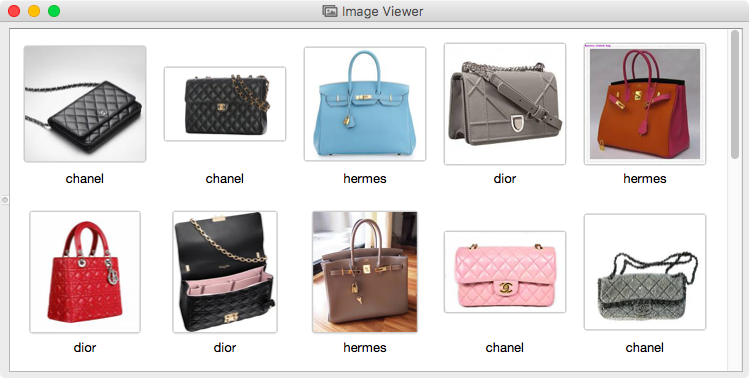
\includegraphics[width=12cm]{slike/torbice.png}
\caption{Ženske torbice različnih proizvajalcev.}
\label{f:torbice}}
\end{figure}

\begin{figure}[htbp]
\centering{
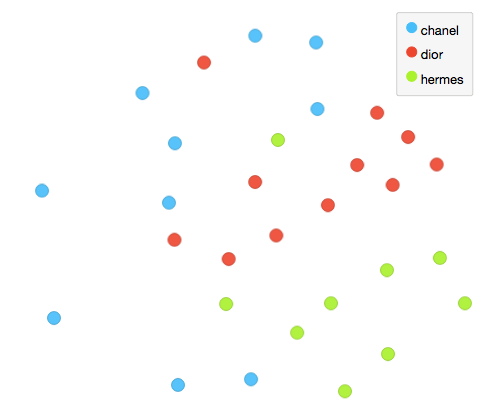
\includegraphics[width=8cm]{slike/torbice-mds.png}
\caption{Predstavitev ženskih torbic s slike~\ref{f:torbice} v dvodimenzionalnem prostoru.}
\label{f:torbice-mds}}
\end{figure}

\section{Metoda glavnih komponent}

Prva, morda tudi najbolj znana metoda za zmanjšanje dimenzij in odkrivanje zanimivih projekcij podatkov je metoda glavnih komponent. Predpostavimo, da imamo dano matriko učnih primerov $X\in\mathbb{R}^{m\times n}$, kjer je $m$ število primerov in $n$ število atributov. Primer $x^{(i)}\in X$, torej $i$-ti primer v učni množici primerov, bo tako opisan z $n$ atributi $x\in\mathbb{R}^{n}$, za katere bomo tu privzeli, da so njihove vrednosti realna števila. V splošnem iščemo projekcije podatkov tako, da atributni zapis primerov z $n$ atributi nadomestimo z atributnim zapisom z $k$ novimi atributi tako, da je $k\ll n$ in da nam novi atributi povedo čim več o primerih iz učne množice.

Pričnimo s $k=1$, torej s projekcijo v eno samo dimenzijo. Dogovorimo se, da bo naša projekcija linearna in da bomo vrednost novega atributa tvorili kot linearno kombinacijo originalnih atributov. Smer projekcijske ravnine oziroma smer premice, na katero bomo projicirali podatke označimo z enotskim vektorjem $u_1$, za katerega torej velja $u_1^\tr u_1=1$.

Naj bo $x^{(i)}$ primer iz učne množice. Njegova projekcija na projekcijsko ravnino je skalar, $u_1 x^{(i)}\in \mathbb{R}$. Naj bo $\bar{x}$ središčna točka podatkov:
%
$$ \mean{x}=\frac{1}{m}\sum_i x^{(i)}$$
%
Projekcija središčne točke na projekcijsko ravnino je $u_1 \mean{x}$. Primeri v učni množici odstopajo od središčne točke, eni bolj, drugi manj. Primere bi želeli projicirati na ravnino tako, da ta odstopanja čim bolj zajamemo, torej, da so tudi v projicirani ravnini čim večja. Povprečno kvadratno odstopanje v projekciji od projekcije središčne točke imenujemo tudi varianca točk v projekciji:
%
$$ \Var(u_1^\tr X^\tr)=\frac{1}{n}\sum_{i=1}^m \big(u_1^\tr x^{(i)}-u_1^\tr\mean{x}\big)^2 $$

Z drugimi besedami, želimo poiskati tak projekcijski vektor $u_1$, ki maksimizira varianco projekcije $\Var(u_1^\tr X^\tr)$. Poigrajmo se malce z enačbo za varianco projekcije:
%
\begin{equation}
  \begin{split}
    \Var(u_1^\tr X^\tr)
    & = \frac{1}{m}\sum_{i=1}^m \big(u_1^\tr x^{(i)}-u_1^\tr\mean{x}\big)^2 \\
    & = \frac{1}{m}\sum_{i=1}^m \big(u_1^\tr x^{(i)} u_1^\tr x^{(i)} - 2 u_1^\tr x^{(i)} u_1^\tr \mean{x} + u_1^\tr \mean{x} u_1^\tr \mean{x} \big)
  \end{split}
\end{equation}
%
Tu upoštevamo, da je $u_1^\tr x$ skalarni produkt dveh vektorjev, in da je transponirana vrednost realnega števila enaka temu številu. Torej je na primer $u_1^\tr x=(u_1^\tr x)^\tr=x^\tr u_1$. Z upoštevanjem tega se nam zgornji izraz primerno poenostavi:
%
\begin{equation}
  \begin{split}
    \Var(u_1^\intercal X^\tr)
    & = \frac{1}{m}\sum_{i=1}^m u_1^\tr \big(x^{(i)} {x^{(i)}}^\tr - 2 x^{(i)} \mean{x}^\tr + \mean{x}~\mean{x}^\tr \big) u_1 \\
    & = u_1^\tr \big( \frac{1}{m}\sum_{i=1}^m (x^{(i)}-\mean{x}) (x^{(i)}-\mean{x})^\tr\big) u_1
  \end{split}
\end{equation}

V oklepaju je kovariančna matrika! Prejšnji stavek smo končali s klicajem zato, ker je kovarianca znan in mnogokrat uporabljan koncept v statistiki in nam pove, kako sta dve naključni spremenljivki povezani. Označimo kovariančno matriko s ${\rm S}$:
\begin{equation}
  {\rm S} = \frac{1}{m}\sum_{i=1}^m (x^{(i)}-\mean{x}) (x^{(i)}-\mean{x})^\tr
\end{equation}

V našem primeru imamo $n$ atributov, kar pomeni, da je kovariančna matrika dimenzije ${\rm S}=\mathbb{R}^{n\times n}$. Zapišimo še enkrat dobljeno enačbo za varianco:
\begin{equation}
  \Var(u_1^\intercal X^\tr) = u_1^\tr {\rm S} u_1
\end{equation}
%
Spomnimo, da je naš namen poiskati projekcijski vektor $u_1$ pri katerem je zgornja varianca maksimalna. Za vektor $u_1$ zahtevamo, da je to enotni vektor (sicer maksimizacija zgornje enačbe ne bi imela smisla, saj bi to dosegli z neskončno dolgim vektorjem $u_1$). Maksimizacijo variance, kjer iščemo ustrezen vektor $u_1$ z omejitvijo $u_1^\tr u_1=1$ rešimo z uporabimo Lagrangeovih multiplikatorjev. Maksimiziramo torej izraz:
%
\begin{equation}
  f(u_1) = u_1^\tr {\rm S} u_1 + \lambda_1(1-u_1^\tr u_1)
\end{equation}
%
V maksimumu bo odvod zgornje enačbe enak nič:
\begin{equation}
  \frac{\partial f(u_1)}{\partial u_1}={\rm S} u_1 - \lambda_1 u_1=0
\end{equation}
%
kar pomeni,
\begin{equation}
  {\rm S} u_1=\lambda_1 u_1
\end{equation}
%
Tu je ${\rm S}$ matrika katere vrednosti poznamo, $u_1$ je vektor, ki ga iščemo, $\lambda_1$ pa skalar. Poznano? Seveda! Zgornjemu pogoju ustreza le tak $u_1$, ki je lastni vektor matrike ${\rm S}$. Ampak korelacijska matrika ima več lastnih vektorjev. Kateri med njimi je pravi? Množimo zgornjo enačbo z $u_1^\tr$:
%
\begin{equation}
  u_1^\tr {\rm S} u_1 = u_1^\tr \lambda_1 u_1=\lambda_1 u_1^\tr u_1=\lambda_1
\end{equation}
%
Na levi je izraz za našo varianco $\Var(u_1^\intercal X^\tr)$, ki jo skušamo maksimizirati. Vemo, da mora biti $u_1$ lastni vektor kovariančne matrike. Skladno z zgornjo enačbo pa sedaj tudi vemo, da je to lastni vektor z najvišjo pripadajočo lastno vrednostjo.

V smeri vektorja $u_1$ se lega naših primerov $X$ v $n$-dimenzionalnem prostoru torej najbolj spreminja, njihova varianca je v tej smeri največja. Z $u_1^\tr X^\tr$ dobimo pravokotno projekcijo vsakega od primerov na to os. S to projekcijo, oziroma legi v smeri $u_1$, smo pojasnili največjo varianco primerov. Kaj še ostane? Vse, kar je pravokotno na smer $u_1$. Največjo varianco na pravokotni hiperravnini pa je ravno v smeri drugega lastnega vektorja, saj je ta pravokoten na $u_1$, to je vektorja, ki ima drugo največjo lastno vrednost. Pojasnjen delež te variance je $\lambda_2$, skupaj pa s pravokotno projekcijo na prvi in drugi lastni vektor pojasnimo $\lambda_1+\lambda_2$ variance množice primerov.

Lastni vektorji kovariančne matrike nam določajo nov koordinatni
sistem, kjer so koordinate, po vrsti, tiste, po katerih se lege točk v
večdimenzionalnem prostoru najbolj spreminjajo, oziroma je njihova
varianca največja. Nove koordinate, urejene skladno z lastnimi vrednostmi vektorjev, imenujemo komponente primerov v novem, transformiranem sistemu. Ker nas bodo zanimale samo te z visokimi deleži razložene variance jih bomo imenovali {\em glavne komponente}.

\begin{figure}[htbp]
\centering{
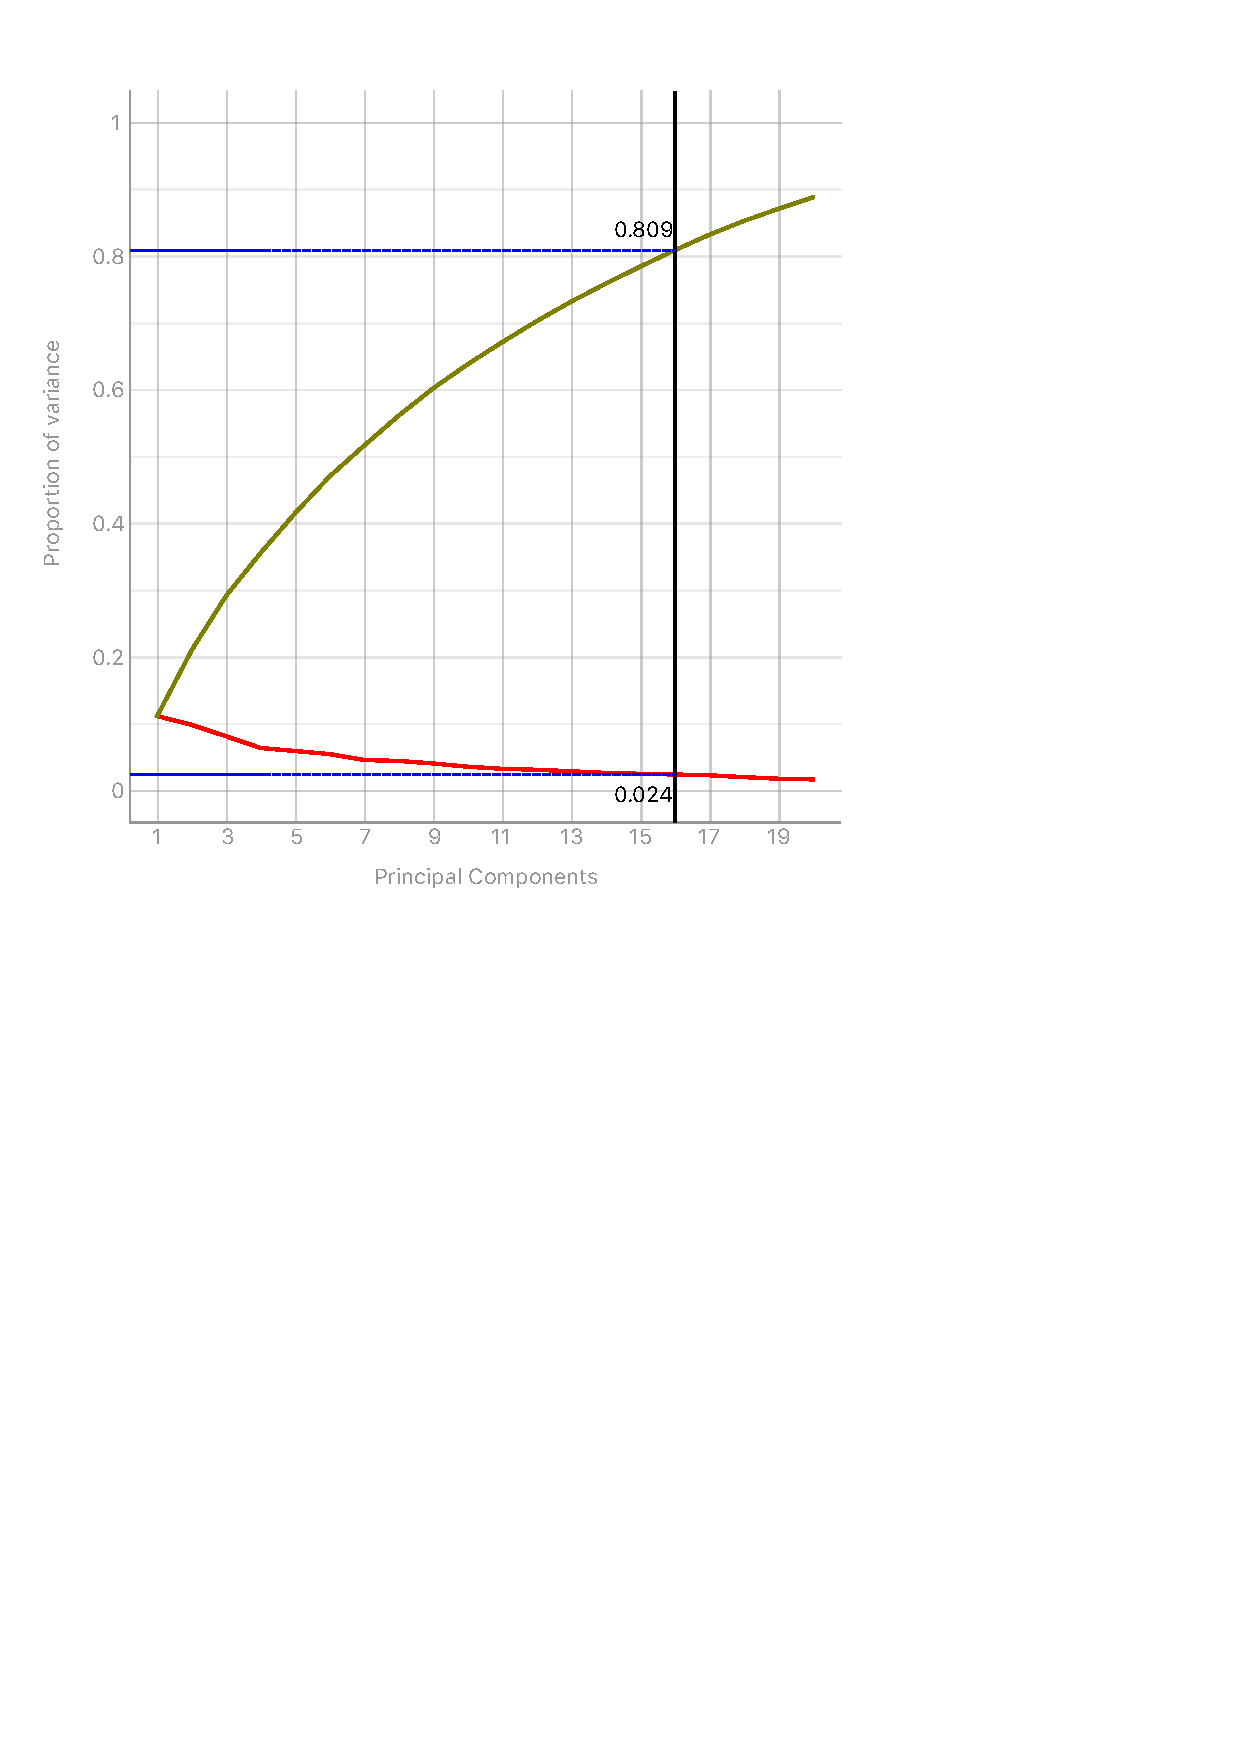
\includegraphics[width=8cm]{slike/scree-diagram.pdf}
\caption{Graf odvisnosti razložene variance od števila glavnih komponent (zgornja črta) za podatke o torbicah iz slike~\ref{f:torbice}.}
\label{f:scree}}
\end{figure}

V splošnem nas zanima, koliko najvišje rangiranih dimenzij v novem
koordinatnem sistemu zares potrebujemo za opis podatkov. Pri tem moramo
seveda določiti, kakšen je naš ciljni delež pojasnjene variance. Tipično
smo zadovoljni, če izbrano število komponent pojasni vsaj $80\%$ skupne variance. Ker skupno varianco poznamo (enaka je vsoti kvadratov razdalj do
centra), je potrebno torej le določiti, koliko začetnih urejenih lastnih
vrednosti moramo sešteti, da njihova vsota predstavlja želeni delež razložene variance. Primer grafa, ki kaže odvisno deleža razložene variance glede na število glavnih komponent kaže slika~\ref{f:scree}.

Pristop glavnih komponent se mnogokrat uporablja tudi samo za namene vizualizacije, kjer primere, opisane z mnogimi atributi, želimo predstaviti v dvodimenzionalni ravnini. Pri tem se moramo seveda zavedati, da prvi dve komponenti razložijo morda le majhen del celotne variance.

Za predstavitev podatkov z glavnimi komponentami je potrebno podatke najprej osrediščiti in nato poiskati kovariančno matriko. Lastni vektorji kovariančne matrike so bazni vektorji novega, transformiranega sistema, njihove lastne vrednosti pa povedo, kakšen delež variance nam razloži posamezna komponenta.

Še praktičen razmislek: v primerih velikega števila atributov bo računanje vseh lastnih vektorjev in vrednosti zamudno. Še posebej, če nas zanima samo projekcija podatkov v dvodimenzionalni prostor. Prvi lastni vektor kovariančne matrike $M$ lahko rajši (hitreje) določimo numerično, s potenčno metodo. Vzamemo nek naključni vektor (npr. $x$), ga transformiramo z matriko $M$ (torej, izračunamo $x\leftarrow M x$), in to ponavljamo do konvergence. Ob vsakem koraku tako dobljeni $x$ normaliziramo, torej, $x\leftarrow \frac{M x}{\norm{M x}}$. Na ta način dobimo lastni vektor. Kako izračunamo pripadajočo lastno vrednost?
\begin{equation}
  M u = \lambda u
\end{equation}

\begin{equation}
  u^\tr M u = u^\tr \lambda u = \lambda u^\tr u = \lambda
\end{equation}

Kako določimo naslednjo komponento? Ena od možnosti je, da uporabimo ravnokar izračunani lastni vektor, nanj projiciramo podatke, te vrednosti odštejemo od podatkov (torej dobimo projekcijo na lastnemu vektorju pravokotno hiperravnino) in za te podatke ponovno izračunamo kovariančno matriko ter s potenčno metodo njej lastni vektor z največjo lastno vrednostjo. V primeru, da potrebujemo več komponent, postopek ustrezno ponovimo.

Za primer, ko nas zanima samo projekcija podatkov v ravnino lahko potenčno metodo namesto na vektorju izvedemo na sistemu dveh vektorjev $U$. Vektorja matrike $U$ morata biti pravokotna. To dosežemo tako, da po vsakem koraku potenčne metode uporabimo Gram-Schmidtovo ortogonalizacijo.

\section{Večrazredno lestvičenje}

Pri zmanjšanju dimenzij nam je lahko cilj, da ohranimo razdalje med posameznimi primeri. Tu predpostavimo, da za vsak par primerov znamo med njimi oceniti razdaljo. Se pravi, če imamo primere predstavljene v atributnem zapisu, potem uporabimo recimo Evklidsko razdaljo ali pa kosinusno podobnost. Lepota tehnike, ki jo bomo predstavili v tem razdelku je, da nas ne zanima, kako je bila podobnost oziroma razdalja med primeri ocenjena. Lahko smo na vhodu na primer imeli tekstovne dokumente, za katere razdaljo recimo izračunamo s kakšno kompresijsko tehniko. Ali pa filme, za katere razdaljo izračunamo z ozirom na njihovo gledanost v spletni sposojevalnici. Ali pa čivke, ki jih primerjamo med sabo glede na to, kdo jih je všečkal.

Naj bo razdalja med primeroma enaka $\delta_{ij}$. Sedaj te primeri vložimo, recimo, v dvodimenzionalno projekcijo tako da vsakemu primeru $i$ pripišemo koordinati $\vect{\theta}^{(i)}=(\theta_1^{(i)},\theta_2^{(i)})$. Želeli bi, da se v njej razdalje ohranjajo, to je, da je projekcijska razdalja, ki naj bo $d_{ij}$, čimbolj podobna originalni razdalji med primeroma. Razdalja primerov v projekcijskem prostoru je:
$$\delta_{ij}=\norm{{\vect{\theta}}^{(i)}-\vect{\theta}^{(j)}}$$

Računalniška izvedba algoritma, ki poišče tako vložitev, imenujemo večrazsežnostno lestvičenje ({\em multidimensional scaling}, MDS). Formalno ciljno funkcijo problema zastavimo tako, da določimo energijo sistema ali napetost ({\em stress}) kot, recimo,
$$J(\mathbf{X}) = \sum_{i\ne j} (d_{ij} - \delta_{ij})^2,$$
kjer je $\mathbf{X}$ trenutni razpored točk, $d_{ij}$ in $\delta_{ij}$ pa trenutna projekcijska in želena razdalja med primeroma $i$ in $j$. Večrazsežnostno lestvičenje poišče razpored $\mathbf{X}$ z najmanjšo napetostjo $J(\mathbf{X})$ oziroma najmanjšo vrednostjo kriterijske funkcije.

Kako minimizirati takšno funkcijo? Analitično ne bo šlo. Za to bi bilo potrebno odvesti $\sigma(\mathbf{X})$ po vseh koordinatah $\theta_1^{(i)}$ in $\theta_2^{(i)}$ in poiskati ničle:
\begin{eqnarray}
  \frac{\partial\sigma({\mathbf{X}})}{\partial \vect{\theta_k}} & = &
  \sum_{j\ne i} \frac{\partial\sigma({\mathbf{X}})}{\partial d_{ij}}\frac{d_{ij}}{\partial \vect{\theta_k}} \nonumber \\
  & = & - \sum_{j\ne i} 2\left(\sqrt{(\theta_1^{(i)}-\theta_1^{(j)})^2+(\theta_2^{(i)}-\theta_2^{(j)})^2}-\delta_{ij}\right) \frac{(\theta_k^{(i)}-\theta_k^{(j)})}{\sqrt{(\theta_1^{(i)}-\theta_1^{(j)})^2+(\theta2^{(i)}-\theta_2^{(j)})^2}} \nonumber \\
& = & - \sum_{j\ne i} 2\left(d_{ij}-\delta_{ij}\right) \frac{(\theta_k^{(i)}-\theta_k^{(j)})}{d_{ij}} \label{eq:mds-grad}
\end{eqnarray}
Pri stotih točkah bi dobili sistem z dvesto takšnimi enačbami; ideji o direktnem napadu se torej raje odpovemo.

Drug, izvedljiv postopek je gradientna metoda: kot pri dosedanjih pristopih z gradientnim spustom (recimo, linearna regresija) izračunamo gradient funkcije kriterijske funkcije $J(\mathbf{X})$. To smo pravzaprav storili že zgoraj. Izberemo si poljuben začetni razpored točk, vstavimo koordinate v odvode, dobimo gradient (vektor odvodov) in se pomaknemo v smeri nasprotni gradientu, se pravi, vse točke pomaknemo v smer, kamor jih potiskajo odvodi. Gradientna metoda bi delovala, vendar ne prav dobro. Bila bi počasna in velikokrat bi nas (lahko) pripeljala le v lokalni minimum.

V svetu optimizacijskih problemov je gradientna metoda le metoda grobe sile, ki jo bomo uporabili, če se ne moremo spomniti ničesar boljšega. Eden od boljših postopkov je ``majorizacija''. Označimo funkcijo, katere minimum iščemo, z $f(x)$. Recimo, da si znamo izmisliti, neko drugo funkcijo $g(x, y)$, ki je stalno večja ali enaka $f(x)$ (torej, za vsak $y$ velja $g(x, y)\ge f(x)$ pri vsakem $x$), v točki $g(x, x)$ pa velja $g(x, x)=f(x)$. Funkcija $g(x, y)$ naj bo takšna, da znamo dobro poiskati vrednost $x$, pri katere doseže minimum. Zdaj lahko počnemo tole: izmislimo si začetni $x_0$. Pri njem, vemo, velja $g(x_0, x_0)=f(x_0)$. Minimiziramo funkcijo $g$ in dobimo nov, boljši $x$ - označimo ga z $x_1$. Vrednost $g(x_1, x_0)$ je manjša ali enaka vrednosti $g(x_0, x_0)$, saj smo minimizirali $g$ po prvem argumentu. Po drugi strani, spet po definiciji funkcije $g$, velja $f(x_1) \le g(x_1, x_0)$. Imamo torej
$$f(x_1) \le g(x_1, x_0) \le g(x_0, x_0) = f(x_0)$$
Postopek ponovimo z $x_1$, da pridelamo naslednji, še boljši $x_2$.

Takšna optimizacija je, tako kot gradientna metoda še vedno iterativna, vendar hitrejša. Koliko hitrejša, je odvisno od tega, kako dobro $g(x, y)$ smo poiskali; $g(x, y)$ se mora čim tesneje prilegati $f(x)$, poleg tega pa jo moramo biti zmožni čim boljše optimizirati.

Algoritem večdimenzionalnega lestvičenja, ki deluje na ta način, se imenuje SMACOF \angl{scaling by majorizing a complicated function}. SMACOF je hitrejši od gradientne metode, dela večje korake in se manjkrat zatakne v lokalnih ekstremih, zato je uporabnejši za (realistične) primere, v katerih je točk veliko.

Za izračun napetosti lahko namesto gornje, naivne formule uporabljamo tudi takšne, ki uteži prispevke parov (predpišemo lahko, za katere pare si še posebej želimo, da bi razdalja ustrezala pravi), poleg tega pa lahko napetost posameznega para normiramo tako, da jo delimo z želeno ali s trenutno razdaljo.

Slika~\ref{f-zoo-mds} kaže zemljevid živali. Razdalje med pari živali so izračunane kot evklidske razdalje med atributi, ki jih opisujejo. Točke, ki predstavljajo živali, smo obarvali glede na vrsto -- vijolični so sesalci, rdeče ptice, oranžno žuželke. Povezani so pari živali, ki so si med seboj najbolj podobne.

\begin{figure}[tbp]
\begin{center}
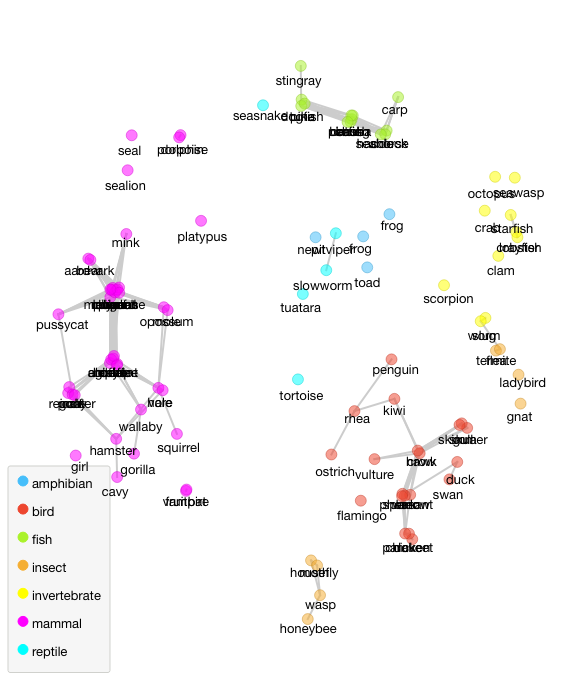
\includegraphics[width=10cm]{slike/zoo-mds.png}
\caption{Zemljevid živali (podatkovna zbirka Zoo). Vrsta živali je označena z barvo. Nekatere oznake so zaradi prekrivanj neberljive in bi razvojnike programa potrebno opozoriti, da v vizualizacijo vključijo optimizacijo postavitve oznak.}
\label{f-zoo-mds}
\end{center}
\end{figure}

Čeprav MDS ni uporabljal podatkov o vrstah živali, so različne vrste na zemljevidu dobro ločene. Vidimo tudi nekaj podobnosti med živalmi: morske sesalce je MDS postavil v bližino rib; dvoživke so blizu rib in nevretenčarjev, predvsem morskih; žuželke so pomešane s ptiči.

Vidimo tudi težavo: žuželke so razdeljene v dve skupini. MDS se je očitno znašel v lokalnem ekstremu, saj bi morale ose in čebele k ostalim žuželkam, vendar bi jih moral optimizacijski postopek peljati okrog ptičev. To se zgodi kar pogosto in pomagamo si tako, da podatke nekoliko potresemo, naključno premaknemo točke, ali pa začnemo celotno optimizacijo znova.

Večrazežnostno lestvičenje je torej postopek, ki vizualizira podatke v obliki zemljevida. Podatki so opisani s seznamom primerov in razdalj med njimi; lastnosti primerov niso potrebne in jih ne znamo upoštevati (razen, če iz le-teh računamo razdalje, kot smo storili pri živalih). Zemljevid je nezanesljiv v tem smislu, da bodo različne naključne začetne postavitve vodile v različne končne slike, a vsaka od njih nam lahko nudi drugačen pogled na podatke. Prav tako je nezanesljiv položaj posameznih točk; dogaja se, da je točka obtičala v lokalnem minimumu, čeprav v resnici ne sodi na to mesto. Takšne točke lahko prepoznamo, če zemljevidu dodamo povezave med najbolj podobnimi pari. Obenem nam takšne povezave pomagajo brati sliko. MDS ne sestavlja gruč, pač pa lahko gruče razberemo sami.

\section{Stohastična vložitev sosedov}

Je lahko še kaj boljšega za vložitev primerov v dvorazsežni prostor kot večrazredno lestvičenje? Oziroma, kaj bi bilo lahko sploh narobe s tehniko MDS? Problem MDS-a je, da se ta osredotoča tako na primere, ki so si v originalnem prostoru blizu, kot tudi na primere, ki so si daleč. MDS skuša ohraniti razdaljo med primeri ne glede na to, kako velika je. Velikokrat pa nas v vizualizacijah zanima samo to, da so primeri, ki so se med seboj podobni, skupaj tudi v projekcijskem prostoru. Torej, ohranjanje razdalje med primere, ki so si med seboj drugačni, nas ne zanima, ali pa nas, recimo, zanima veliko manj kot ohranjanje bližine med seboj podobnih primerov.

Metoda SNE \angl{stochastic neighbor embedding}, ki smo jo tu poslovenili v stohastično vložitev sosedov, temelji na verjetnostni oceni podobnosti dveh primerov. Za primera $i$ in $j$ oziroma njuni vektorski predstavitvi $x^{(i)}$ in $x^{(j)}$ določimo verjetnost $p_{j|i}$, da bi za primer $i$ izbrali soseda $j$, če bi sosede izbirali skladno z Gaussovo verjetnostno porazdelitvijo, ki je centrirana v $x^{(i)}$:
\begin{equation}
  p_{j|i}=\frac{\exp(-\norm{x^{(i)}-x^{(j)}}^2/2\sigma_i^2)}
  {\sum_{k\neq i}\exp(-\norm{x^{(i)}-x^{(k)}}^2/2\sigma_i^2)}
\end{equation}
kjer je $\sigma_i$ varianca Gaussove porazdelitve za točko $i$. Ker nas zanimajo samo modeliranje podobnosti med različnimi točkami, je $p_{i|i}$ enaka nič. Zanima nas vložitev teh primerov v projekcijski prostor, kjer bo lega primerov kot pri MDS določena z vektorji $\vect{\theta}^{(i)}$ in bomo podobno kot zgoraj, le tokrat za projekcijski prostor, sosednost predstavili z verjetnostjo $q_{j_i}$.

Označimo verjetnostne porazdelitve preko vseh sosedov z za primer $i$ in za originalni prostor z $P_i$ in za projekcijski prostor z $Q_i$. Naša želja je, da bi bili ti porazdelitvi med sabo čim bolj podobni. Ker ti dve verjetnostni porazdelitve favorizirajo bližnje primere oziroma so za te verjetnosti visoke, podobnost porazdelitev $P_i$ in $Q_i$ pomeni, da je projekcija ohranila bližnje primere za primer $i$. Mera, ki pove, kako zvesto $q_{j|i}$ sledi $p_{j|i}$ je Kullback-Leibler-jeva divergenca, katere vsoto po primerih želimo minimizirati. Kriterijska funkcija je zato:
\begin{equation}
  J(\vect{\Theta}) = \sum_i KL(P_i\ ||\ Q_i)=\sum_i\sum_j p_{j|i}\log\frac{p_{j|i}}{q_{j|i}}
\end{equation}
Zaradi nesimetričnosti Kullback-Leibler-jeva divergence bodo napake obravnavane nesimetrično: cena za v projekciji oddaljene točke, ki bi sicer morale biti blizu (majhen $q$ in velik $p$) bo večja kot za točke, ki so bližje v projekciji, a bi sicer morale biti daleč (velik $q$ in majhen $p$). Metoda SNE primarno ohranja sosednost.

Med parametri kriterijske funkcije nam je ostal nedoločen še $\sigma_i$, parameter verjetnostne porazdelitve za primer $i$. Metoda SNE ga določi skladno z lokalno gostoto primerov tako, da je za gostejše okolice $\sigma_i$ primerno manjši.

Da bi določili vložitev moramo poiskati lege primerov $\vect{\theta}^{(i)}$ v projekcijskem prostoru. To lahko vnovič storimo z gradientnim sestopom:
%
\begin{equation}
\nonumber
\pd{\vect{\Theta}}{\vect{\theta}^{(i)}}=
  2\sum_j(p_{j|i}-q_{j|i}+p_{i|j}-q_{i|j})(\vect{\theta}^{(i)}-\vect{\theta}^{(j)})
\end{equation}
%
Gradient (popravek) bo večji pri večji razliki med $p$ in $q$ (prvi člen v produktu) med primeroma in bo potekal v smeri vektorja med primeri (drugi člen produkta).

Danes je predvsem znana ``popravljena'' verzija metode SNE, ki jo imenujemo $t$-SNE \angl{t-distributed stochastic neighbor embedding}. V njej Gaussovo porazdelitev za projekcijski prostor zamenjajo s Studentovo $t$-porazdelitvijo, ki ima daljši rep. S to zamenjavo $t$-SNE dovoli, da so primeri, ki so v srednji okolici v originalnem prostoru lahko daleč stran v projekcijski ravnini. Tehnika namesto pogojnih verjetnosti uporablja združene verjetnosti, in simetrično oceno sosednosti za primere v originalnem prostoru,
%
\begin{equation}
  \nonumber
  p_{ij}=\frac{\exp(-\norm{x^{(i)}-x^{(j)}}^2/2\sigma^2)}
  {\sum_{k\neq l}\exp(-\norm{x^{(k)}-x^{(l)}}^2/2\sigma^2)}
\end{equation}
%
ter za projekcijski prostor
\begin{equation}
  \nonumber
  q_{ij}=\frac{(1+\norm{x^{(i)}-x^{(j)}}^2)^{-1}}
  {\sum_{k\neq l}(1+\norm{x^{(k)}-x^{(l)}}^2)^{-1}}
\end{equation}
%
Tudi tu porazdelitvi primerjamo s Kullback-Leiblerjevo divergenco,
\begin{equation}
  \nonumber
  J(\vect{\Theta}) = \sum KL(P\ ||\ Q)=\sum_i\sum_j p_{ij}\log\frac{p_{ij}}{q_{ji}}
\end{equation}
za katero poiščemo gradient:
%
\begin{equation}
  \nonumber
  \pd{\vect{\Theta}}{\vect{\theta^{(i)}}} = 4\sum_j(p_{ij}-q_{ij})
\frac{(\vect{\theta^{(i)}}-\vect{\theta^{(j)}})}{(1+\norm{\vect{\theta^{(i)}}-\vect{\theta^{(j)}}}^2)}.
\end{equation}
Zgornja enačba je po strukturi presenetljivo podobna enačbi~\ref{eq:mds-grad}  za gradient pri večrazrednem lestvičenju, kar je glede na drugačen način izpeljave nekoliko presenetljivo, glede na intuitivno razumevanje cilja obeh projekcij pa morda sploh ne. Glavna razlika obeh metod je seveda ocenjevanje razdalj oziroma pojmovanje, oziroma bolje uteževanje sosednosti. Če pri večrazrednem lestvičenju razdalja ni utežena, je pri metodi SNE in izvedenkah stopnja sosednosti eksponencialno padajoča funkcija.

Metoda $t$-SNE je v zadnjih letih postala izjemno popularna. Njen problematičen del je predvsem v parametrizaciji (iskanje prave vrednosti za parametre Gaussove distribucije) in v relativni počasnosti metode oziroma pripadajočega gradientnega pristopa.

\section{FreeViz}

Denimo, da imamo primere, ki so opisani z atributi, za vsak primer pa je podan tudi razred. Zemljevid takšnih podatkov bi sicer lahko narisali z večrazežnostnim lestvičenjem, kot smo to storili pri živalih, vendar bi tako zanemarili podatke o pripadnosti razredom. Poleg tega si pri takšnih podatkih navadno želimo imeti model, s katerim bomo lahko uvrščali nove podatke; MDS nam tega ne omogoča.

Želimo si torej metodo, ki vsaki točki priredi njeno mesto na podlagi vrednosti njenih atributov, pri čemer naj bo mesto določeno tako, da bodo primeri iz istega razreda blizu eden drugemu.

Primer takšne metode je FreeViz. FreeViz je linearna projekcija. Če imajo primeri $n$ atributov, bomo rekli, da se nahajajo v $n$-dimenzionalnem prostoru; vsak primer je točka in njene koordinate so pač vrednosti atributov. Primere, kot smo to počeli do sedaj, opišemo z vektorjem-kolono $\vect{x} = [x_1, x_2, \ldots, x_n]^\tr$. Vsakemu atributu ustreza ena dimenzija, njej pa en bazni vektor v originalnem prostoru primerov. Linearne projekcije so določene s slikami baznih vektorjev. Naj bodo torej $\vect{a_1}, \vect{a}_2, \ldots, \vect{a}_n$ slike baznih vektorjev, $\vect{a}_i = [a_{i,x}, a_{i,y}]^\tr$. Zložimo  jih v matriko, $\vect{A} = [\vect{a}_0 | \vect{a}_1 | \ldots | \vect{a}_k]$. Projekcija primera $\vect{x}$ je tako enaka $\vect{\theta} = \vect{A}\vect{x}$. Naloga FreeViz-a je poiskati dobro projekcijsko matriko $\vect{A}$.

Kaj pomeni dobro matriko? Določiti moramo funkcijo, ki jo želimo optimizirati. Za razliko od MDSa tokrat ne bomo definirali energije, temveč silo (torej v resnici ne definiramo funkcije, ki jo želimo optimizirati, temveč njen gradient). Točki, ki ustrezata primeroma iz istega razreda, se bosta privlačili, točke, ki ustrezajo primerom iz različnih razredov, se bodo odbijale. Za razliko od tega, česar smo navajeni iz fizike, bodo privlačne sile naraščale z razdaljo. To je smiselno zato, ker je točke, ki so izgubljene nekje daleč od svojih, težko privleči mimo vseh točk, ki so jim na poti, zato jih bomo vlekli z veliko silo. Po drugi strani pa dveh točk iz istega razreda, ki so že prišle blizu ena drugi, nima smisla tlačiti še bližje. Z odbojnimi silami je ravno nasprotno: točke različnih razredov, ki so si blizu skupaj želimo na vsak način spraviti narazen. Točk različnih razredov, ki so že daleč narazen, pa nima smisla še bolj odbijati. Zato bodo odbojne sile z razdaljo padale.

Naj bo torej ${\bm F_{ij}}$ sila, s katero projiciran primer $j$ deluje na točko $i$; definiramo jo lahko recimo, tako, da za točke istega razreda narašča in za točke različnih razredov pada premosorazmerno z razdaljo (po želji pa lahko izberemo tudi kvadrat ali kako drugo primerno funkcijo razdalje). Naj bo ${\bm F_i} = \sum_{j\ne i} {\bm F_{ij}}$ vsota vseh sil na točko $i$. Sprememba potencialna energija projicirane točke je določena s silo in spremembo lege točke:
\begin{equation}
  \nonumber
  dE_i=-\vect{\bm F_i}^\tr \vect{\theta^{(i)}},
\end{equation}
%
sprememba energije celotnega sistema pa
\begin{equation}
  \nonumber
  dE=-\sum_i\vect{\bm F_i}^\tr\vect{\theta^{(i)}},
\end{equation}

Naše točke, primeri, so fiksni, spreminja pa se projekcijska matrika $\vect{A}$. Ker je projekcija primerov določena z $\vect{\theta}^{(i)}=\vect{A}\vect{x}^{(i)}$, so spremembe lege v projekcijski ravnini plod sprememb v projekcijski matriki:
\begin{equation}
  \nonumber
  \vect{d\theta}^{(i)}=\vect{dA}\vect{x}^{(i)}
\end{equation}
%
Ko se spreminja projekcijska matrika, se spreminja potencialna energija sistema:
\begin{equation}
  \begin{split}
    \nonumber
    dE = & -\sum_i \vect{F}_i^\tr \vect{d\theta}^{(i)} \\
    \nonumber
    = & -\sum_i \vect{F}_i^\tr \vect{dA}\vect{x}^{(i)}
  \end{split}
\end{equation}
%

Iščemo gradient, ki nam pove, kako sprememba projekcije $i$-tega primera vpliva na spremembe energije sistema. Ta znaša $\vect{F}_i{{x}^{(i)}}^\tr$, 
oziroma združeni gradient, ki pove, kako sprememba projekcije vseh primerov vpliva na skupno energijo sistema:
\begin{equation}
  \begin{split}
    \frac{\partial E}{\partial \vect{A}} = & \sum_i\vect{F}_i{{x}^{(i)}}^\tr \\
 = & {\bm F} {\bm X},
  \end{split}
\end{equation}
%
Algoritem FreeViz prične z neko naključno matriko $\vect{A}$ in potem v vsakem koraku izračuna sile na točke v projekcijski ravnini in gradiente ter projekcijo matriko ustrezno spremeni. Postopek ponavlja do konvergence.

\begin{figure}[tbp]
\begin{center}
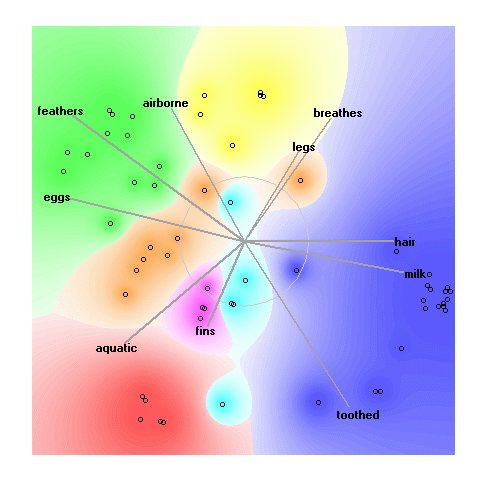
\includegraphics[width=12cm]{slike/zoo-freeviz.png}

\includegraphics[width=12cm]{slike/zoo-legenda.png}
\caption{Projekcija FreeViz iz podatkov o živalih}
\label{f-zoo-freeviz}
\end{center}
\end{figure}


Rezultat takšne projekcije na podatkih o živalih vidimo na sliki~\ref{f-zoo-freeviz}. Iz nje lahko, če znamo, razberemo veliko lastnosti podatkov. Na sliki so različna področja obarvana glede na prevladujočo živalsko vrsto - sesalci so modri, ribe rdeče in tako naprej. Osi ustrezajo atributom; smer osi nakazuje regijo, živalsko vrsto, ki jo sugerira visoka vrednost tega atributa. Vsi atributi, razen števila nog, so binarni, torej v tem primeru recimo dlake in zobje kažejo, da je žival verjetno sesalec. Iz osi torej razberemo povezavo med atributi in razredi, vidimo, katera živalska vrsta je značilna za posamezno lastnost, oziroma, katere lastnosti so značilne za posamezno živalsko vrsto.

FreeViz lahko beremo -- podobno kot MDS -- kot zemljevid. Ptiči in žuželke so si med seboj podobne; oboji letijo, zato v njuno smer kaže atribut {\em airborne}. Prav tako so si podobne ribe in dvoživke.

Vidimo lahko tudi podobnosti med atributi: kosmate živali dajejo mleko; živali, ki letajo, imajo perje, živali, ki plavajo, plavuti in živali, ki dihajo, noge. Obenem razberemo tudi glavne osi, po katerih lahko ločimo živali: žival bodisi daje mleko, bodisi vali jajca (vodoravna os) in je vodna žival s plavutmi ali pa dihajoča žival z nogami.

Osi, ki predstavljajo atribute, so različno dolge; čim pomembnejši je atribut, tem daljša je pripadajoča os. Manj pomembni atributi, katerih osi bi bile krajše od kroga v sredini, zaradi preglednosti niso narisani.

Končno, FreeViz je mogoče uporabljati tudi za uvrščanje primerov. Nov primer, katerega vrednosti atributov poznamo, razreda pa ne, lahko projeciramo in preverimo, v katero regijo je padel. Če v modro, je najbrž sesalec, če v zeleno, ptič\ldots

Ob uporabi FreeViza se moramo zavedati, da gre le za projekcijo v dvodimenzionalni prostor. Vse, kar vidimo, ni nujno resnično. Določeni atributi so morda tam, kjer so, samo zato, ker nekje pač morajo biti. Če uporabljamo FreeViz za iskanje vzorcev, moramo z njim dobljene vzorce preveriti, po možnosti na povsem novih podatkih ali pa jih primerjati z ekspertnim predznanjem o problemu.

FreeViza ne smemo uporabiti, kadar je število atributov primerljivo številu primerov ali celo večje. V tem primeru je mogoče kar analitično poiskati neskočno število rešitev, pri katerih so vse sile enake 0, razpored točk pa je v tem primeru nesmiseln. Slabost FreeViza je tudi, da v osnovi temelji na gradientni metodi in postane pri velikem številu točk počasen. Na lokalne ekstreme pa je, kakor je videti, dokaj neobčutljiv.


\cleardoublepage


\endinput

\section{Singularni razcep}

Oglejmo si podatke šestih filmskih zanesenjakov in njihovih ocenah filmov v tabeli~\ref{t:romance-sf}. Že na prvi pogled lahko opazimo, da imam najbrž dve skupini ocenjevalcev in dve skupini filmov. Metka, Neža, Maja in Tina ne marajo znanstvene fantastike in jim je bolj blizu romantika. Alojz in Gašper pa rajši gledata znanstveno fantastiko in jima romantični filmi niso prav blizu.

\begin{table}
\begin{tabular}{rcccccc}
\toprule
 & Cvetje & Titanic & Harry & Sally & Alien & Prometheus \\
\midrule
Metka & 1 & 2 & 1 & 0 & 0 \\
Neža & 2 & 4 & 2 & 0 & 0 \\
Maja & 3 & 5 & 3 & 0 & 0 \\
Tina & 5 & 10 & 5 & 0 & 0 \\
Alojz & 0 & 1 & 0 & 1 & 2 \\
Gašper & 0 & 0 & 0 & 2 & 4 \\
\bottomrule
\end{tabular}
\label{t:romance-sf}
\end{table}

Skupine pa nismo našli samo pri ocenjevalcih. Že zgoraj smo filme razvrstili v dve skupini, in te uganili iz kratkih nazivov filmov. Pa lahko te skupine, torej skupine uporabnikov in skupine filmov, razpoznamo algoritmično? Lahko podatke, ki jih imamo zgoraj, predstavimo v neki zgoščeni obliki, kjer bi iz zgoščenega zapisa bilo možno prepoznati skupine in interakcijo med ocenjevalci in filmi. Opazimo, recimo, da vsaka od vrstic v naši ocenjevalni tabeli izvira od enega od spodnjih vrstičnih vektorjev, ki ga moramo ustrezno pomnožiti z neko konstanto. 
% 
$$
\begin{bmatrix}
1 & 1 & 1 & 0 & 0 \\
0 & 0 & 0 & 1 & 1 \\
\end{bmatrix}
$$
Lahko take vektorje prepoznamo iz podatkov? Tehnika, ki jo bomo za to uporabili, se imenuje {\em singularni razcep}. Podatki iz tabele~\ref{t:romance-sf} so že sicer zapisani v atributni obliki in jih lahko torej predstavimo v matriki $A=\mathbb{R}^{m\times n}$. To matriko v splošnem s singularnim razcepom zapišemo kot produkt treh matrik:
\begin{equation}
A = U\Sigma V^\tr
\end{equation}
kjer so:
\begin{itemize}
\item leva singularna matrika $U\\mathbb{R}^{m\times r}$, ki $m$ objektov v vrsticah predstavi v $r$-dimenzionalnem prostoru,
\item desna singularna matrika 
\end{itemize}



\end{document}
